% !TeX document-id = {de0f7ffc-4c3c-4f3a-bd65-453318d6d0bb}
% !TeX TXS-program:compile = txs:///pdflatex/[--shell-escape]
%% bare_conf.tex
%% V1.4b
%% 2015/08/26
%% by Michael Shell
%% See:
%% http://www.michaelshell.org/
%% for current contact information.
%%
%% This is a skeleton file demonstrating the use of IEEEtran.cls
%% (requires IEEEtran.cls version 1.8b or later) with an IEEE
%% conference paper.
%%
%% Support sites:
%% http://www.michaelshell.org/tex/ieeetran/
%% http://www.ctan.org/pkg/ieeetran
%% and
%% http://www.ieee.org/

%%*************************************************************************
%% Legal Notice:
%% This code is offered as-is without any warranty either expressed or
%% implied; without even the implied warranty of MERCHANTABILITY or
%% FITNESS FOR A PARTICULAR PURPOSE! 
%% User assumes all risk.
%% In no event shall the IEEE or any contributor to this code be liable for
%% any damages or losses, including, but not limited to, incidental,
%% consequential, or any other damages, resulting from the use or misuse
%% of any information contained here.
%%
%% All comments are the opinions of their respective authors and are not
%% necessarily endorsed by the IEEE.
%%
%% This work is distributed under the LaTeX Project Public License (LPPL)
%% ( http://www.latex-project.org/ ) version 1.3, and may be freely used,
%% distributed and modified. A copy of the LPPL, version 1.3, is included
%% in the base LaTeX documentation of all distributions of LaTeX released
%% 2003/12/01 or later.
%% Retain all contribution notices and credits.
%% ** Modified files should be clearly indicated as such, including  **
%% ** renaming them and changing author support contact information. **
%%*************************************************************************


% *** Authors should verify (and, if needed, correct) their LaTeX system  ***
% *** with the testflow diagnostic prior to trusting their LaTeX platform ***
% *** with production work. The IEEE's font choices and paper sizes can   ***
% *** trigger bugs that do not appear when using other class files.       ***                          ***
% The testflow support page is at:
% http://www.michaelshell.org/tex/testflow/



\documentclass[conference]{IEEEtran}
% Some Computer Society conferences also require the compsoc mode option,
% but others use the standard conference format.
%
% If IEEEtran.cls has not been installed into the LaTeX system files,
% manually specify the path to it like:
% \documentclass[conference]{../sty/IEEEtran}





% Some very useful LaTeX packages include:
% (uncomment the ones you want to load)


% *** MISC UTILITY PACKAGES ***
%
%\usepackage{ifpdf}
% Heiko Oberdiek's ifpdf.sty is very useful if you need conditional
% compilation based on whether the output is pdf or dvi.
% usage:
% \ifpdf
%   % pdf code
% \else
%   % dvi code
% \fi
% The latest version of ifpdf.sty can be obtained from:
% http://www.ctan.org/pkg/ifpdf
% Also, note that IEEEtran.cls V1.7 and later provides a builtin
% \ifCLASSINFOpdf conditional that works the same way.
% When switching from latex to pdflatex and vice-versa, the compiler may
% have to be run twice to clear warning/error messages.






% *** CITATION PACKAGES ***
%
\usepackage{cite}
% cite.sty was written by Donald Arseneau
% V1.6 and later of IEEEtran pre-defines the format of the cite.sty package
% \cite{} output to follow that of the IEEE. Loading the cite package will
% result in citation numbers being automatically sorted and properly
% "compressed/ranged". e.g., [1], [9], [2], [7], [5], [6] without using
% cite.sty will become [1], [2], [5]--[7], [9] using cite.sty. cite.sty's
% \cite will automatically add leading space, if needed. Use cite.sty's
% noadjust option (cite.sty V3.8 and later) if you want to turn this off
% such as if a citation ever needs to be enclosed in parenthesis.
% cite.sty is already installed on most LaTeX systems. Be sure and use
% version 5.0 (2009-03-20) and later if using hyperref.sty.
% The latest version can be obtained at:
% http://www.ctan.org/pkg/cite
% The documentation is contained in the cite.sty file itself.






% *** GRAPHICS RELATED PACKAGES ***
%
\ifCLASSINFOpdf
 \usepackage[pdftex]{graphicx}
% declare the path(s) where your graphic files are
 \graphicspath{{graphics/}}
% and their extensions so you won't have to specify these with
% every instance of \includegraphics
 \DeclareGraphicsExtensions{.pdf,.jpeg,.png}

 \usepackage[export]{adjustbox} 
\else
% or other class option (dvipsone, dvipdf, if not using dvips). graphicx
% will default to the driver specified in the system graphics.cfg if no
% driver is specified.
% \usepackage[dvips]{graphicx}
% declare the path(s) where your graphic files are
% \graphicspath{{../eps/}}
% and their extensions so you won't have to specify these with
% every instance of \includegraphics
% \DeclareGraphicsExtensions{.eps}
\fi
% graphicx was written by David Carlisle and Sebastian Rahtz. It is
% required if you want graphics, photos, etc. graphicx.sty is already
% installed on most LaTeX systems. The latest version and documentation
% can be obtained at: 
% http://www.ctan.org/pkg/graphicx
% Another good source of documentation is "Using Imported Graphics in
% LaTeX2e" by Keith Reckdahl which can be found at:
% http://www.ctan.org/pkg/epslatex
%
% latex, and pdflatex in dvi mode, support graphics in encapsulated
% postscript (.eps) format. pdflatex in pdf mode supports graphics
% in .pdf, .jpeg, .png and .mps (metapost) formats. Users should ensure
% that all non-photo figures use a vector format (.eps, .pdf, .mps) and
% not a bitmapped formats (.jpeg, .png). The IEEE frowns on bitmapped formats
% which can result in "jaggedy"/blurry rendering of lines and letters as
% well as large increases in file sizes.
%
% You can find documentation about the pdfTeX application at:
% http://www.tug.org/applications/pdftex


\usepackage{color}


% *** MATH PACKAGES ***
%
\usepackage{amsmath}
\usepackage{amssymb}
% A popular package from the American Mathematical Society that provides
% many useful and powerful commands for dealing with mathematics.
%
% Note that the amsmath package sets \interdisplaylinepenalty to 10000
% thus preventing page breaks from occurring within multiline equations. Use:
%\interdisplaylinepenalty=2500
% after loading amsmath to restore such page breaks as IEEEtran.cls normally
% does. amsmath.sty is already installed on most LaTeX systems. The latest
% version and documentation can be obtained at:
% http://www.ctan.org/pkg/amsmath





% *** SPECIALIZED LIST PACKAGES ***
%
%\usepackage{algorithmic}
% algorithmic.sty was written by Peter Williams and Rogerio Brito.
% This package provides an algorithmic environment fo describing algorithms.
% You can use the algorithmic environment in-text or within a figure
% environment to provide for a ing algorithm. Do NOT use the algorithm
% floating environment provided by algorithm.sty (by the same authors) or
% algorithm2e.sty (by Christophe Fiorio) as the IEEE does not use dedicated
% algorithm float types and packages that provide these will not provide
% correct IEEE style captions. The latest version and documentation of
% algorithmic.sty can be obtained at:
% http://www.ctan.org/pkg/algorithms
% Also of interest may be the (relatively newer and more customizable)
% algorithmicx.sty package by Szasz Janos:
% http://www.ctan.org/pkg/algorithmicx




% *** ALIGNMENT PACKAGES ***
%
\usepackage{array}
% Frank Mittelbach's and David Carlisle's array.sty patches and improves
% the standard LaTeX2e array and tabular environments to provide better
% appearance and additional user controls. As the default LaTeX2e table
% generation code is lacking to the point of almost being broken with
% respect to the quality of the end results, all users are strongly
% advised to use an enhanced (at the very least that provided by array.sty)
% set of table tools. array.sty is already installed on most systems. The
% latest version and documentation can be obtained at:
% http://www.ctan.org/pkg/array


% IEEEtran contains the IEEEeqnarray family of commands that can be used to
% generate multiline equations as well as matrices, tables, etc., of high
% quality.




% *** SUBFIGURE PACKAGES ***
%\ifCLASSOPTIONcompsoc
%  \usepackage[caption=false,font=normalsize,labelfont=sf,textfont=sf]{subfig}
%\else
%  \usepackage[caption=false,font=footnotesize]{subfig}
%\fi
% subfig.sty, written by Steven Douglas Cochran, is the modern replacement
% for subfigure.sty, the latter of which is no longer maintained and is
% incompatible with some LaTeX packages including fixltx2e. However,
% subfig.sty requires and automatically loads Axel Sommerfeldt's caption.sty
% which will override IEEEtran.cls' handling of captions and this will result
% in non-IEEE style figure/table captions. To prevent this problem, be sure
% and invoke subfig.sty's "caption=false" package option (available since
% subfig.sty version 1.3, 2005/06/28) as this is will preserve IEEEtran.cls
% handling of captions.
% Note that the Computer Society format requires a larger sans serif font
% than the serif footnote size font used in traditional IEEE formatting
% and thus the need to invoke different subfig.sty package options depending
% on whether compsoc mode has been enabled.
%
% The latest version and documentation of subfig.sty can be obtained at:
% http://www.ctan.org/pkg/subfig




% *** FLOAT PACKAGES ***
%
\usepackage{fixltx2e}
% fixltx2e, the successor to the earlier fix2col.sty, was written by
% Frank Mittelbach and David Carlisle. This package corrects a few problems
% in the LaTeX2e kernel, the most notable of which is that in current
% LaTeX2e releases, the ordering of single and double column floats is not
% guaranteed to be preserved. Thus, an unpatched LaTeX2e can allow a
% single column figure to be placed prior to an earlier double column
% figure.
% Be aware that LaTeX2e kernels dated 2015 and later have fixltx2e.sty's
% corrections already built into the system in which case a warning will
% be issued if an attempt is made to load fixltx2e.sty as it is no longer
% needed.
% The latest version and documentation can be found at:
% http://www.ctan.org/pkg/fixltx2e


%\usepackage{stfloats}
% stfloats.sty was written by Sigitas Tolusis. This package gives LaTeX2e
% the ability to do double column floats at the bottom of the page as well
% as the top. (e.g., "\begin{figure*}[!b]" is not normally possible in
% LaTeX2e). It also provides a command:
%\fnbelowfloat
% to enable the placement of footnotes below bottom floats (the standard
% LaTeX2e kernel puts them above bottom floats). This is an invasive package
% which rewrites many portions of the LaTeX2e float routines. It may not work
% with other packages that modify the LaTeX2e float routines. The latest
% version and documentation can be obtained at:
% http://www.ctan.org/pkg/stfloats
% Do not use the stfloats baselinefloat ability as the IEEE does not allow
% \baselineskip to stretch. Authors submitting work to the IEEE should note
% that the IEEE rarely uses double column equations and that authors should try
% to avoid such use. Do not be tempted to use the cuted.sty or midfloat.sty
% packages (also by Sigitas Tolusis) as the IEEE does not format its papers in
% such ways.
% Do not attempt to use stfloats with fixltx2e as they are incompatible.
% Instead, use Morten Hogholm'a dblfloatfix which combines the features
% of both fixltx2e and stfloats:
%
% \usepackage{dblfloatfix}
% The latest version can be found at:
% http://www.ctan.org/pkg/dblfloatfix

% helpful macros
% helpful macros

\usepackage{xspace}

\newcommand{\hide}[1]{}
\setlength{\marginparwidth}{2cm}
%\newcommand{\comment}[1]{\marginpar{\footnotesize #1}}
%\newcommand{\comment}[1]{}
\newcommand{\comment}[1]{\textcolor{red}{[#1]}}
\renewcommand{\tilde}[0]{$\sim$}
\newcommand{\us}[0]{$\mu s$}

\newcommand{\fig}[1]{Fig.~\ref{#1}\xspace}
\newcommand{\tbl}[1]{Table~\ref{#1}\xspace}
\newcommand{\sect}[1]{Section~\ref{#1}\xspace}

% affiliation shorthand
\newcommand{\ee}[0]{$^{1}$}
\newcommand{\cs}[0]{$^{2}$}
\newcommand{\eecs}[0]{$^{1,2}$}
\definecolor{code-bgnd}{gray}{0.95}
\newcommand{\code}[1]{\colorbox{code-bgnd}{\texttt{#1}}}


% *** NON FLOAT MINIPAGE ***
\makeatletter
\let\MYcaption\@makecaption
\makeatother

\usepackage{caption}
\usepackage[font=footnotesize]{subcaption}

\usepackage[inline]{enumitem}

\makeatletter
\let\@makecaption\MYcaption
\makeatother


% *** PDF, URL AND HYPERLINK PACKAGES ***
%
\usepackage{url}
% url.sty was written by Donald Arseneau. It provides better support for
% handling and breaking URLs. url.sty is already installed on most LaTeX
% systems. The latest version and documentation can be obtained at:
% http://www.ctan.org/pkg/url
% Basically, \url{my_url_here}.



% *** MINTED COLORED CODE ***
\usepackage{minted} % Required to display colored code properly
%hack for minted to get rid of syntax error boxes
\makeatletter
\AtBeginEnvironment{minted}{\dontdofcolorbox}
\def\dontdofcolorbox{\renewcommand\fcolorbox[4][]{##4}}
\makeatother
\usepackage[utf8]{inputenc}

% *** Do not adjust lengths that control margins, column widths, etc. ***
% *** Do not use packages that alter fonts (such as pslatex).         ***
% There should be no need to do such things with IEEEtran.cls V1.6 and later.
% (Unless specifically asked to do so by the journal or conference you plan
% to submit to, of course. )


% *** Custom Frame ***
\usepackage{mdframed}

% So footnotes for figures are properly placed
\usepackage{afterpage}

% correct bad hyphenation here
\hyphenation{op-tical net-works semi-conduc-tor}

% for left justification of text
\usepackage{ragged2e}

% for footnotes inside tables
\usepackage{threeparttable}


\begin{document}
	%
	% paper title
	% Titles are generally capitalized except for words such as a, an, and, as,
	% at, but, by, for, in, nor, of, on, or, the, to and up, which are usually
	% not capitalized unless they are the first or last word of the title.
	% Linebreaks \\ can be used within to get better formatting as desired.
	% Do not put math or special symbols in the title.
	\title{DFiant: A Dataflow Hardware Description Language}
	
	% author names and affiliations
	% use a multiple column layout for up to three different
	% affiliations
\hide{
	\author{\IEEEauthorblockN{Oron Port}
		\IEEEauthorblockA{Electrical Engineering\\
			Technion -- Israel Institute of Technology\\
			Email: soronpo@campus.technion.ac.il}
		\and
		\IEEEauthorblockN{Yoav Etsion}
		\IEEEauthorblockA{Electrical Engineering and Computer Science\\
			Technion -- Israel Institute of Technology\\
			Email: yetsion@tce.technion.ac.il}}
}

\newcommand{\halfbox}[1]{\makebox[0.5\columnwidth]{#1}}
\newcommand{\fullbox}[1]{\makebox[\textwidth]{#1}}
\author{
  \halfbox{Oron Port\ee} \halfbox{Yoav Etsion\eecs}\\
  {\normalsize \halfbox{Electrical Engineering\ee} \halfbox{Computer Science\cs}}\\
  {\normalsize \fullbox{Technion -- Israel Institute of Technology}}\\
  {\normalsize \halfbox{soronpo@campus.technion.ac.il} \halfbox{yetsion@technion.ac.il}}
}

	% conference papers do not typically use \thanks and this command
	% is locked out in conference mode. If really needed, such as for
	% the acknowledgment of grants, issue a \IEEEoverridecommandlockouts
	% after \documentclass
	
	% for over three affiliations, or if they all won't fit within the width
	% of the page, use this alternative format:
	% 
	%\author{\IEEEauthorblockN{Michael Shell\IEEEauthorrefmark{1},
	%Homer Simpson\IEEEauthorrefmark{2},
	%James Kirk\IEEEauthorrefmark{3}, 
	%Montgomery Scott\IEEEauthorrefmark{3} and
	%Eldon Tyrell\IEEEauthorrefmark{4}}
	%\IEEEauthorblockA{\IEEEauthorrefmark{1}School of Electrical and Computer Engineering\\
	%Georgia Institute of Technology,
	%Atlanta, Georgia 30332--0250\\ Email: see http://www.michaelshell.org/contact.html}
	%\IEEEauthorblockA{\IEEEauthorrefmark{2}Twentieth Century Fox, Springfield, USA\\
	%Email: homer@thesimpsons.com}
	%\IEEEauthorblockA{\IEEEauthorrefmark{3}Starfleet Academy, San Francisco, California 96678-2391\\
	%Telephone: (800) 555--1212, Fax: (888) 555--1212}
	%\IEEEauthorblockA{\IEEEauthorrefmark{4}Tyrell Inc., 123 Replicant Street, Los Angeles, California 90210--4321}}
	
	
	
	
	% use for special paper notices
	%\IEEEspecialpapernotice{(Invited Paper)}
	
	
	
	
	% make the title area
	\maketitle
	
	% As a general rule, do not put math, special symbols or citations
% in the abstract
\begin{abstract}
Today's dominant hardware description languages (HDLs), namely Verilog and VHDL, rely on limited register-transfer-level (RTL) constructs. These constructs tightly couple design functionality with timing requirements and target-device constraints. As hardware designs and device architectures become increasingly more complex, these dominant HDLs yield verbose and unportable code.
To raise the level of abstraction, several high-level synthesis (HLS) tools were introduced, usually based on software languages such as C. Unfortunately, designing hardware with sequential software language semantics comes at a price; the designer loses the ability to control hardware construction and data scheduling, which is crucial in many design use-cases. 

In this paper we further extend DFiant, a Scala-based HDL that uses the dataflow model to decouple functionality from implementation constraints.
DFiant's frontend enables functional bit-accurate hardware description, while maintaining a complete timing-agnostic and device-agnostic code. DFiant bridges the gap between software programming and hardware construction, driving an intuitive functional object oriented code into a high-performance hardware implementation.

For a proof of concept, we implemented a compiler frontend for DFiant, which transforms DFiant code into a dataflow graph, and a preliminary auto-pipelining backend, which maps the graph into synthesizable Verilog code. We further implemented two test cases in DFiant: an Advanced Encryption Standard cipher block and an IEEE-754 floating point multiplier. We compared both test cases against modern design flows. Our results demonstrate that DFiant can greatly simplify hardware designs yet still maintain competitive performance.
\end{abstract}

%We defined a new language from the ground up, borrowing concepts from hardware, dataflow and software languages. The result is a strongly-typed, purely synthesizable extendable language frontend, fit for both general-purpose and high level hardware description.
	

	% no keywords
	
	
	% For peer review papers, you can put extra information on the cover
	% page as needed:
	% \ifCLASSOPTIONpeerreview
	% \begin{center} \bfseries EDICS Category: 3-BBND \end{center}
	% \fi
	%
	% For peerreview papers, this IEEEtran command inserts a page break and
	% creates the second title. It will be ignored for other modes.
	%\IEEEpeerreviewmaketitle
	
	
	
	\section{Introduction}
The register-transfer level (RTL) programming model paved the road for Verilog and VHDL to flourish as the leading hardware description languages (HDLs). That road, however, is steadily nearing its end as both hardware designs and devices become increasingly more complex. While the software world is striving for a "write once, run anywhere" programmability, the complexity of an RTL design implementing a given functionality may vary greatly across different FPGA and ASIC devices that incorporate various technologies and core components. Moreover, minor requirement changes may lead to significant redesigns, since RTL abstraction tightly couples functionality with timing constraints. For example, registers serve various roles such as preserving a state, pipelining and balancing a data path, deriving timed signals from an input clock, and synchronizing an input signal. This coupling between functionality, timing constraints, and device constraints leads to verbose and unportable RTL designs. 

\begin{figure}[h]
	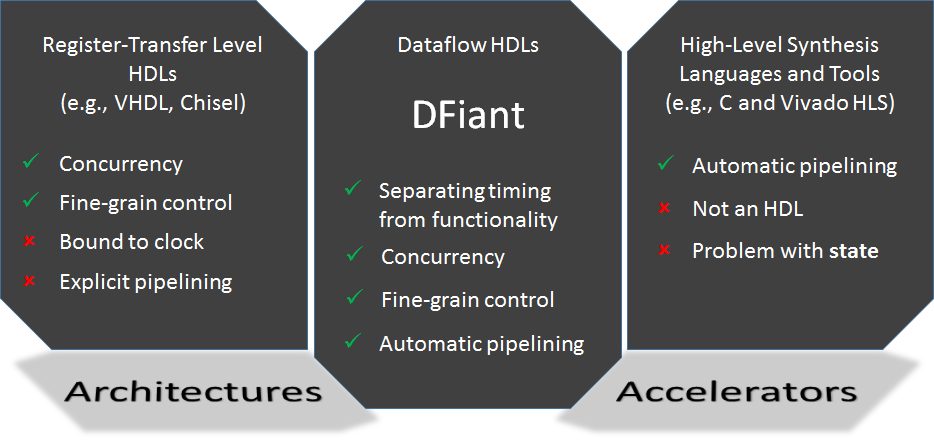
\includegraphics[width=\linewidth]{graphics/teaser}
	\caption{DFiant bridges the gap}
	\label{fig:teaser}
\end{figure}

Ongoing efforts to bridge this hardware programmability gap~\cite{Kapre2016, Nane2016, Windh2015} can be largely split into two classes: high-level synthesis (HLS) tools and high-level RTL (HL-RTL) languages.
On the one hand, HLS tools (such as Vivado~\cite{Vivado2012}, Catapult~\cite{graphics2008catapult}, and others~\cite{Kavvadias2013, synphony2015}) rely on programming languages like C and incorporate auto-pipelining and optimization mechanisms to make hardware accelerators accessible for non-hardware engineers. While this approach is successful in algorithmic acceleration domains, such languages carry von Neumann sequential semantics and thus hinder construction of parallel hardware, which is crucial for hardware design~\cite{Zhao2017}. Moreover, some trivial periodic hardware operations (like toggling a LED) are unbearably difficult to implement in HLS languages.
On the other hand, HL-RTL languages (such as Chisel~\cite{Bachrach2012}, Bluespec~\cite{nikhil2004bluespec}, PyRTL~\cite{Clow2017}, and others~\cite{Charles2016, Liu2017, jiang2018mamba, decaluwe2004myhdl, CxLang2014, Lockhart2014}) aim to enhance productivity by introducing new hardware generation constructs and semantics but do not abstract away register-level description (even Bluespec, which uses concurrent guarded atomic actions, assumes rules complete within a single clock cycle). Therefore, HL-RTL designs are still subjected to the \emph{"tyranny of the clock"}~\cite{Sutherland2012} and are bound to specific timing and target constraints.

In this paper we propose dataflow-based HDL constructs that abstract away registers and clocks. We further introduce DFiant\footnote{A preliminary version of DFiant was first introduced as a poster. The reference was removed for blind review.}, a Scala-embedded HDL that utilizes these dataflow constructs to decouple functionality from implementation constraints. DFiant brings together constructs and semantics from dataflow~\cite{le1986signal, Thuau1991, gurd1985manchester, arvind1992id}, hardware, and software programming languages to enable truly portable and composable hardware designs. The dataflow model offers implicit concurrency between independent paths while freeing the designer from explicit register placement that binds the design to fixed pipelined paths and timing constraints.

\begin{figure*}[t]
	\centering
	\captionsetup{justification=centering}
	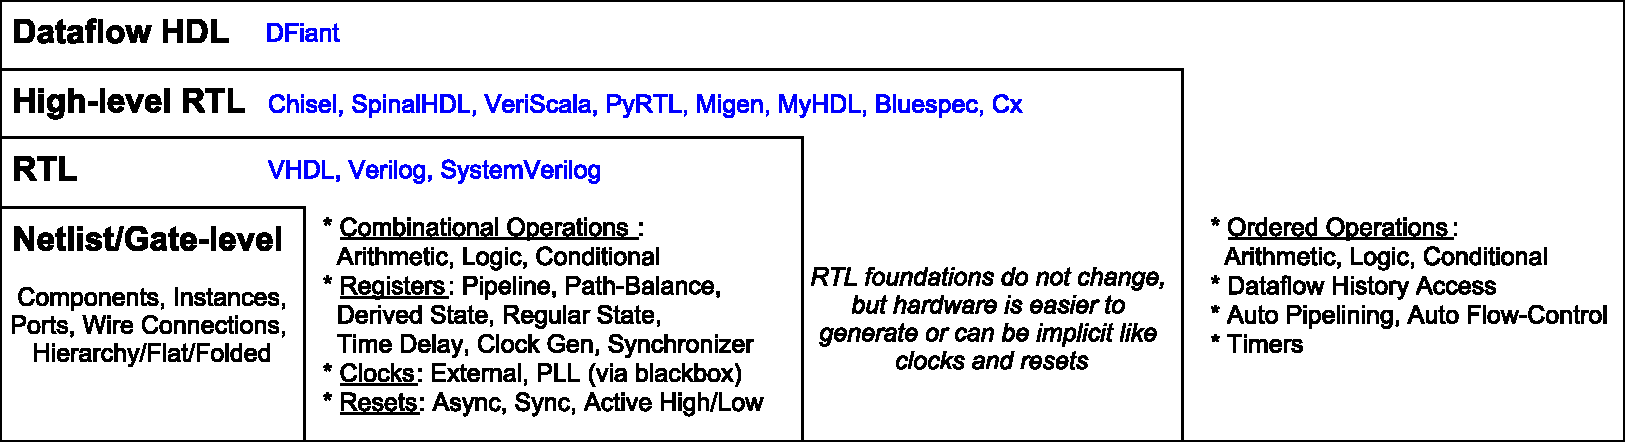
\includegraphics[width=\linewidth]{graphics/motivation.pdf} 
	\captionof{figure}{HDL abstraction layer summary (lowest=netlist, highest=dataflow)\\ Each layer subsumes the capabilities of the layer below it. Dataflow constructs replace RTL registers with their true functionality (e.g., state) or inserts them implicitly (e.g., pipelining). }
	\label{fig:motivation}
\end{figure*}

Recent related dataflow-for-hardware efforts are the Maxeler framework~\cite{Pell2011} and its MaxJ Java-based programming language, the OpenDF framework~\cite{bhattacharyya2008opendf} which is based on the CAL actor language~\cite{eker2003cal}, and CAPH~\cite{serot2011implementing}. MaxJ indeed shares common traits with DFiant, but it is tailored for its target hardware framework and is not designed to be a general purpose HDL. Both OpenDF and CAPH share similar goals with our work, but they use actors and networks to describe hardware, which is completely different than a conventional HDL composition based on component instances and port connections.

This work focuses on applying dataflow principles through the DFiant language and compiler. DFiant is \emph{not} an HLS language, nor is it an RTL language. Instead, DFiant is an HDL that provides abstractions beyond the RTL behavioral model, which reduce verbosity and maintain portable code. Since DFiant is implemented as a Scala library, it offers a rich type safe ecosystem alongside its own hardware-focused type system (e.g., bit-accurate dataflow types, input/output port types). The library performs two main tasks: first, the frontend compilation, which enforces the type-safe rule-system and constructs a dataflow dependency graph; and second, the backend compilation, which translates the graph into a pipelined RTL code and a TCL constraints file. The resulting code can be synthesized using commercial tools. 

The remainder of this paper is organized as follows. The next section details the motivation behind the dataflow HDL abstractions, and Section~\ref{sec:dfiant} which provides a general overview of the DFiant HDL language. 
Section~\ref{sec:evaluation} describes our evaluation of the DFiant language and compiler, and, finally, Section~\ref{sec:conclusion} concludes the paper.


%Interactions between DFiant types lead to hardware construction, while non-DFiant types (e.g. Integer) are considered as constants. 
 

  
  \begin{table*}[t]
  \begin{threeparttable}
  \captionof{table}{Data Scheduling Semantics Example Function, $f$: Definition and Implementations}
  \label{tbl:DataSchedDefImpl}
  \setlength\tabcolsep{1.5pt}
  \begin{tabular}{|c|c|c|c|c|}
  \hline 
  \textbf{Formal Definition} & \textbf{Functional Drawing} & \textbf{C++ Impl.}\tnote{†} & \textbf{VHDL Impl.\tnote{‡}} & \textbf{DFiant Impl.} \\ 
  \hline
	\begin{minipage}[b]{0.23\linewidth}
    {\fontsize{7}{8}\selectfont
    \begin{equation}    
      \nonumber
      \begin{aligned}
        &f:(i_{n})_{n\in \mathbb{N}}\rightarrow (a_n,b_n,c_n,d_n)_{n\in \mathbb{N}}\\ 
        &\triangleq\left\{
        \begin{split}
          a_k & = i_k + 5 \\
          b_k & = a_k * 3 \\
          c_k & = a_k + b_k \\
          d_k & = i_k - 1 \\
        \end{split}\right.k\geq 0 \\
        \\
      \end{aligned}
    \end{equation}
    }
	\end{minipage}
  &
	\begin{minipage}[b][3.1cm][c]{0.18\linewidth}
    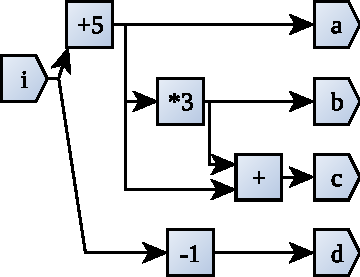
\includegraphics[width=\linewidth]{graphics/fFuncDraw.pdf}
  \end{minipage}%
  &
	\begin{minipage}[b]{0.18\linewidth}
		\begin{minted}[autogobble,tabsize=2,fontsize=\fontsize{7}{8}\selectfont]{c}
      void f(int i,
             &a,&b,&c,&d){ 
      
      
        a = i + 5;
        b = a * 3;
      
        c = a + b;
        d = i - 1;

      }
		\end{minted}
	\end{minipage}
	&
	\begin{minipage}[b]{0.18\linewidth}
		\begin{minted}[autogobble,tabsize=2,fontsize=\fontsize{7}{8}\selectfont]{vhdl}
      f : process(clk)
      begin 
        if rising_edge(clk)
        begin
          a <= i + 5;
          b <= a * 3;
          â <= a;--cyc delay
          c <= â + b;
          d <= i - 1;
        end; 
      end process;
		\end{minted}
	\end{minipage}
	&
	\begin{minipage}[b]{0.19\linewidth}
		\begin{minted}[autogobble,tabsize=2,fontsize=\fontsize{7}{8}\selectfont]{scala}
      def f(i : DFSInt[32]) = 
      {
      
      
        val a = i + 5
        val b = a * 3
      
        val c = a + b
        val d = i - 1
        (a,b,c,d) //tuple of
      }           //four
		\end{minted}
	\end{minipage}
  \\
  \hline
  \end{tabular}
  \begin{tablenotes}
    \item [†] Some type annotations were removed for brevity.
    \item [‡] \textbf{â} represents a clock cycle delay of \textbf{a}.
  \end{tablenotes}
  \end{threeparttable}
\end{table*}%

\section{Concurrency and Data Scheduling Abstractions}
\label{sec:concurrency_abstractions}

Concurrency and data scheduling abstractions rely heavily on language semantics. In this section, we explore semantics of three distinctively different languages: C++, VHDL, and DFiant. 

Consider the function $f$ and its implementations, as detailed in Table \ref{tbl:DataSchedDefImpl}. Despite similar code appearance, the semantics are very different, as depicted in Fig. \ref{fig:DataSchedGraph}. The following subsections qualify these semantics.


\subsection{C++ Semantics}
Sequential programming models, such as C++, do not have concurrent semantics. Data scheduling order is set by \textit{code statement order}, and cannot be pipelined\footnote{We only observe language semantics. Out-of-order or multi-processor executions may still apply.}. HLS utilities extends these languages with \code{pragma} directives that change semantics. We observe the C++ \code{f} implementation as follows:

\begin{figure}[t]
  \vspace*{-6ex}
  \centering
  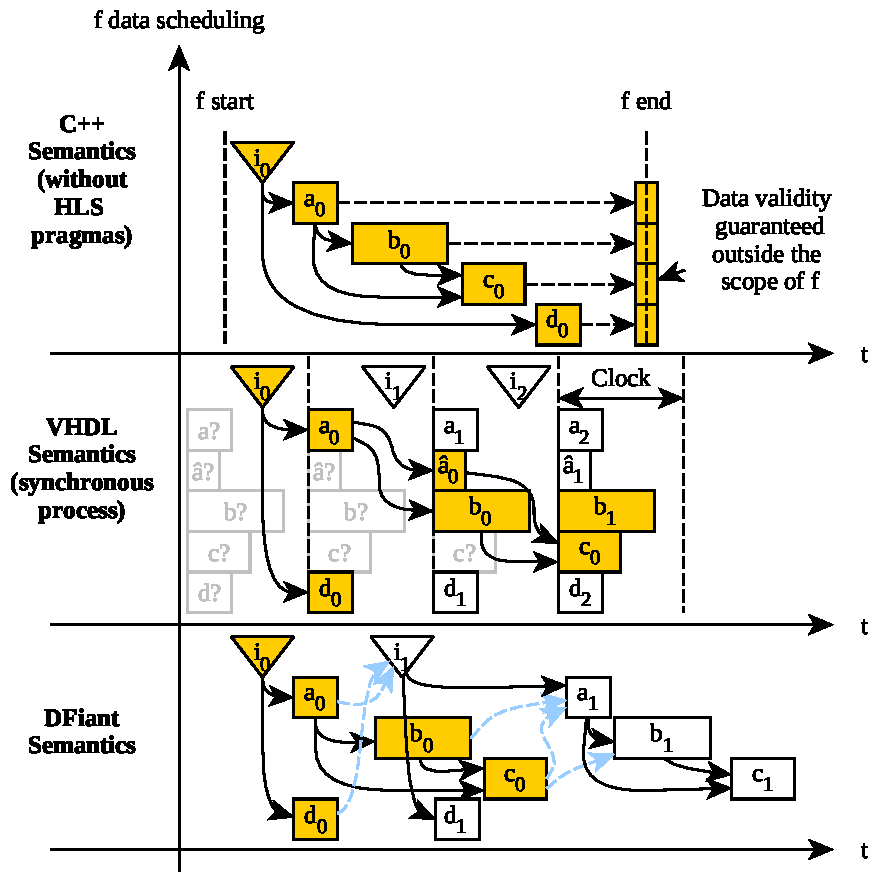
\includegraphics[width=\linewidth]{graphics/DataScheduling.pdf}
  \captionof{figure}{$f$ data scheduling semantics in C++, VHDL, and DFiant}
  \label{fig:DataSchedGraph}
\end{figure}

\begin{enumerate}
  \item All statements are variable assignments.
  \item \code{d} is independent of \code{a}, \code{b}, and \code{c}, but cannot be scheduled concurrently. Additionally, \code{a} cannot be safely read until \code{f} ends. Proper pragmas allow dataflow analysis and function inlining to overcome these limitations.
  \item Time between/of the data operations is unconstrained. The code does not restrict the functional requirement and will maintain correctness for every hardware synthesis fitting its semantics. 
\end{enumerate}  

\subsection{VHDL Semantics}
The RTL programming model is concurrent. Data scheduling is manual and clock-bound, while the order is set by the \textit{assignment cycle-time}. VHDL process semantics are different for \textit{signals} and \textit{variables}: signals are updated when the process ends, while variables are updated instantly. When embedded in a signal edge-detection conditional construct, both signals and variables can be interpreted as registers, depending on the context. We observe the VHDL \code{f} implementation as follows:

\begin{enumerate}
  \item All statements are synchronous signal assignments with an explicit single-clock dependency. Clocked \code{f} imposes time restrictions to $f$. Although this implementation does not contradict the formal definition of $f$, its correctness is guaranteed solely under these restrictions.
  \item A latency balancing register added to maintain correctness of the \code{c} assignment pipeline\footnote{We can use VHDL variable to avoid latency balancing, by forming a combinational circuit.}. 
  \item Data is scheduled for every clock cycle, thus creating a pipeline. Each output signal is valid at a different time. Invalid outputs may be accessed, since VHDL has no implicit $guard$ semantics. More hardware is required to match the output cycle-latencies, and implement explicit guards.
  \item The implementation is very fragile and has limited reusability. Foremost, VHDL process construct alone is not reusable, and requires an \textit{entity-architecture} encapsulation for structural instantiation. Additionally, \code{f} is tightly-coupled to \code{clk} timing and logic propagation delay. The slightest change in requirements or target device can lead to a painful redesign. 
\end{enumerate}

\subsection{DFiant Semantics}
DFiant has a dataflow programming model. Data scheduling order, or \textit{token-flow}, is set by the \textit{data dependency}. Essentially, the DFiant semantics schedules all independent dataflow expressions concurrently, while dependent operations are synthesized into a guarded FIFO-styled pipeline. Dataflow branches are implicitly forked and joined. Unused nodes, semantically, always consume tokens, and are discarded during compilation. We observe the DFiant \code{f} implementation as follows:

\begin{enumerate}
  \item All expressions are dataflow variable declarations.
  \item Concurrency is implicit, and \code{f} is coded intuitively, in a sequential manner, since dataflow dependency is oblivious to statement order. 
  \item All scheduling is implicitly guarded by its dependencies. For example, \code{a} is forked into both \code{b} and \code{c} operations, while \code{c} joins branches from \code{a} and \code{b}.
  It is impossible to read an invalid result or an old result (without extending semantics further).
  \item DFiant semantics are intuitive: data is consumed only when it is ready and can be accepted by all receiving nodes, while back-pressure prevents data loss. 
\end{enumerate} 
   

\subsection{Semantics Comparison}
Comparing DFiant and VHDL, it is evident that DFiant is less verbose and has better semantics for code reuse. The given VHDL implementation is a private case for DFiant, since it is only one of many possible solutions, while DFiant relies on its compiler to generate hardware in respect to design constraints. DFiant prevents \code{f} users from reading invalid values, while in VHDL it must be programmed explicitly. Bluespec and Chisel have similar semantics to VHDL, thus suffer from related limitations (e.g., explicit pipelining). Fortunately, they both can provide guarded types that prevent invalid data use.

Comparing DFiant and C++, we observe that C++ HLS tools rely on code analysis and pragma directives to change the semantics of their sequential code, while DFiant has its own dataflow type system that guarantees its seamless concurrent semantics. Consequently, C++ HLS tools limit language constructs and hierarchies which are not supported by the analysis algorithms (e.g., recursion), in contrary to DFiant which supports all finite Scala constructs (e.g., finite generation loops and recursions). 
%We believe that constraint directives should not change semantics but refine them.

Contrarily, tandem operations are described more naturally in C++, and loops are utilized to describe repetitive dependent tasks. With proper pragmas, C++ loop iterations can run concurrently, but since they can also run sequentially, loops, and nested loops especially, may be semantically confusing. For this reason, DFiant does not support loops, same as VHDL (hardware generation loops are supported), and opts for state machine semantics to describe sequential operations. %We cover state in the next section. 
%We further compare DFiant against other HLS tools and languages in Section \ref{sec:related_work}. 



%  \section{Register and State Abstraction}
\label{sec:state_abstractions}
\begin{table*}
  \begin{threeparttable}
  \captionof{table}{State Semantics Example Function, $g$: Definition and Implementations}
	\label{tbl:StateExDefImpl}
	\setlength\tabcolsep{1.5pt}
  \begin{tabular}{|c|c|c|c|c|}
  \hline 
  \textbf{Formal Definition} & \textbf{Functional Drawing} & \textbf{C++ Impl.}\tnote{†}~\tnote{‡} & \textbf{VHDL Impl.}\tnote{‡} & \textbf{DFiant Impl.} \\ 
  \hline
	\begin{minipage}[b][3.2cm][c]{0.21\linewidth}
    {\fontsize{8}{8}\selectfont
		\begin{equation}
			\nonumber
      \begin{split}
			&g:(i_{n})_{n\in \mathbb{N}}\rightarrow (a_n,b_n,c_n)_{n\in \mathbb{N}}\\  
      &\triangleq\left\{
      \begin{aligned}
      a_k &= i_k+5 & k\geq 0\\ 
      b_k &= i_k+i_{k-1} & k>0 \\   
      b_k &= i_k+0  & k=0 \\
      c_k &= i_k+c_{k-1} & k>0  \\ 
      c_k &= i_k+0 & k=0
      \end{aligned} 
      \right.
      \end{split}
		\end{equation}
    }
	\end{minipage}
  &
	\begin{minipage}[b][3.2cm][c]{0.18\linewidth}
    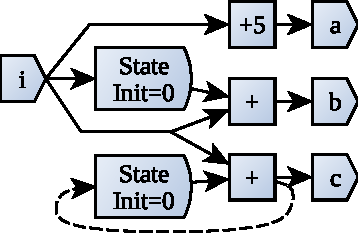
\includegraphics[width=\linewidth]{graphics/gFuncDraw.pdf}
  \end{minipage}%
  &
	\begin{minipage}[b]{0.14\linewidth}
		\begin{minted}[autogobble,tabsize=2,fontsize=\fontsize{8}{8}\selectfont]{c}
      void g(int i,
             &a,&b,&c){
        static int î=0;
        static int C=0;
        
        a = i + 5;
        b = i + î;
        î = i;
        c = i + C;
        C = c;
      }
		\end{minted}
	\end{minipage}
	&
	\begin{minipage}[b]{0.21\linewidth}
		\begin{minted}[autogobble,tabsize=2,fontsize=\fontsize{8}{8}\selectfont]{vhdl}
      g : process(clk)
        variable î : integer:=0;
      begin
        if rising_edge(clk)
        begin
          a <= i + 5;
          b <= i + î;
          î := i;
          c <= i + c;
        end; 
      end process;
			\end{minted}
	\end{minipage}
	&
	\begin{minipage}[b]{0.23\linewidth}
		\begin{minted}[autogobble,tabsize=2,fontsize=\fontsize{8}{8}\selectfont]{scala}
      def g(i : DFSInt[32]) = 
      {
        
        
        
        val a = i + 5
        val b = i + i.init(0).prev
        val c = DFSInt[32]
        c := i + c //prev optional
        (a,b,c) //tuple of three
      }
		\end{minted}
	\end{minipage}
  \\
  \hline
  \end{tabular}
  \begin{tablenotes}
    \item [†] Some type annotations were removed for brevity.
    \item [‡] \textbf{î} and \textbf{C} represent previous state values of \textbf{i} and \textbf{c}, respectively.
  \end{tablenotes}
  \end{threeparttable}
\end{table*}%

In the previous section we compared implementations of a pure (stateless) function, $f$. Typical designs, however, possess a state that is implemented via clocked registers. Registers have other functional roles, such as pipelining a data path, deriving timed signals from an input clock, and synchronizing an input signal. We believe that by avoiding explicit register use, we can design without, or very little, clock dependency. 

In this section we classify various register use-cases, and present their DFiant functional counterpart. The classifications are divided into three main categories: \textit{synchronous technology backend}, \textit{synchronous technology interface}, and \textit{state}. For the state classification, we also explore an impure function, $g$, and compare its implementation in VHDL, C++, and DFiant (see Table~\ref{tbl:StateExDefImpl}).

%Clocked registers have various functional roles, yet all appear the same in modern HDL designs. 
%The main reason is that devices have very small number of IO ports, measurable in the hundreds, while modern designs process trillions of bps. Designs are This, of course, forces existance of state, since pure functions must receive all inputs  . Therefore, it is impossible to avoid state in a full (\textit{top}) system hardware description. 
%When HLS abstract away the clock, it is left to the code analysis to classify what variable hold state.

\subsection{Synchronous Technology Backend}
Registers are often forced upon the design due to a synchronous technology choice. Since they are unrelated to the functional requirement, DFiant has no constructs to express them, and relies on its compiler to implement them properly based on the functional requirements and design constraints.
We differentiate between the following backend register uses:
\subsubsection{Pipelining}
DFiant auto-pipelines the design by inserting registers to split long combinational paths. The amount of pipelining is determined by designer-specified constraints, such as the maximum path cycle latency, or the maximum propagation delay between registers.
\subsubsection{Synchronizers}
Sampling clock domain crossing (CDC) or asynchronous signals is exposed to metastability. Synchronizers, often composed of registers, are used to mitigate its effect and bring the design to the proper reliability. Since we aspire for a clockless design frontend, we want the synchronizers to be implicit. Currently, DFiant only supports a single clock backend, and does not require synchronizers. Further research may explore other backend options.

\subsection{Synchronous Technology Interface}
Functional design requirements are often accompanied by synchronous input/output (IO) timing constraints such as clocked protocol interfaces or real-time restrictions. However, these constraints only effect the interface, and are unrelated to the design core. To maximize design portability, we apply legacy constructs solely in the periphery, while keeping the design core coded in dataflow. DFiant exposes a frontend bridge across legacy RTL constructs and its dataflow types. We differentiate between the following synchronous signaling:
\subsubsection{External IO and Blackbox Interfaces}
External IOs that are exposed to the top design hierarchy, or blackboxes that are exposed to the internal design core, may impose synchronous protocols (e.g., data is valid one clock cycle after address is set). DFiant supports legacy RTL constructs to synchronously interface external IOs and instantiate blackboxes. 
%We implemented a preliminary interface between DFiant and Chisel, allowing us to tap into Chisel's hardware generation and cycle accurate simulations.
\subsubsection{Timers}
Timers are design constructs for outputting real-time signals, or creating derivations of timed signal inputs. For example, a target device is fed by a 100MHz clock and we want to output a UART stream at 10Mbps or toggle a led at 1Hz. Instead of directly applying registers or clock generation components, we can create functional representation of their timed use-cases. Currently, DFiant supports timers with legacy RTL constructs. This work may be expanded to include functional timers.

\subsection{State}
State occurs when we require access to (previous) values which are no longer available on a function's inputs (e.g., cumulative sum or a state-machine's state). Table~\ref{tbl:StateExDefImpl} introduces a state function, $g$, and its implementation in C++, VHDL, and DFiant. The C++ implementation uses the \code{static} keyword to create variables that maintain the history of \code{i} and \code{c}. Because a static variable saves its value for every call of \code{g}, the C++ implementation cannot be used in the same design more than once. The VHDL implementation invokes registers (behaviorally) to save the state. Unfortunately, registers not only save the state, but also enforce specific cycle latencies. Furthermore, both C++ and VHDL declare additional variables and place extra assignments just to save the state. DFiant overcomes all these issues and in a less cumbersome way.

The DFiant state abstraction is achievable via the \code{.prev} construct, to summon the previous dataflow variable value, and also the construct \code{.init(value)}, to create an initialized dataflow variable. The \code{:=} assignment operation is available for a mutable dataflow variable such as \code{c} (see Section~\ref{sec:mutability}). The creation of \code{c} carries within it an implicit assignment \code{c := c.init(0).prev}, which makes the next assignment of \code{c}, \code{c := i + c}, equivalent to \code{c := i + c.init(0).prev}. This is possible due to the following semantics: \textit{previous values change at the end of the DFiant code} (similarly to signal update semantics in VHDL processes). One advantage is that the code resembles its RTL counterparts, but less verbose. Another advantage is that any type of state component, like the Muller C-element\cite{muller1957theory}, can be applied with DFiant as a frontend (note that the functional drawing in Table~\ref{tbl:StateExDefImpl} has no register drawn).

%entire design or process loop semantics. DFiant variables are implicitly static.
%Functionally a register is a memory with a single write port and unlimited

We differentiate between two kinds of state: \textit{derived state}, and \textit{regular state}. Addressable memory pools also hold state, but we currently classify them as blackboxes. %Future work may provide dedicated functional abstractions for such components as well.

\subsubsection{Derived State} 
A derived state is a state whose current output value is \textit{independent} of its previous value. For example, calculating output \code{b} of function \code{g} requires summoning previous value of \code{i}. 

\subsubsection{Regular State} 
A regular state is a state whose current output value is \textit{dependent} of its previous state value. For example, the cumulative sum output, \code{c}, of function \code{g} is dependent on the old sum value. 

The two types of state differ heavily in performance improvement when the design is pipelined. A path from \code{i} to \code{b} can produce a token for every clock tick, and if we pipeline the addition operation to increase the maximum frequency, the maximum throughput will increase as well. Contrarily, a path from \code{i} to \code{c} also depends on the previous value of \code{c}, and if we pipeline the addition operation of that path, the extra latency may even decrease the throughput. Furthermore, \code{i} is forked into several paths, and  abides by the slowest path throughput. 

Regular state causes bottlenecks in many systems. For instance, a processor's program counter (PC) register manifests as a regular state. The processor pipeline can only be improved thanks to a speculative mechanism that predicts the next PC value to prefetch instructions (e.g., PC+4 for a branch-not-taken prediction). In case of a miss-prediction, other mechanisms take place. Further research may expand DFiant's abstractions, and solve such problems functionally.

%\subsubsection{Speculated State} 
%A speculated state is a regular state that can generate a new speculative value when the actual next value is unavailable.

%In some cases a regular state limits the throughput too much. For example, a program counter (PC) register for a microprocessor pipeline. If we state dependent on the PC as a regular state, it won't be possible for the pipeline to handle more than one instruction at a time. A known solution for this is to speculate on the next value of PC (good guess is branch not taken). If we guessed wrong the pipeline should ignore the prefetched instructions and restart from where the branch occurred. This allows us to generate new speculative tokens of PC, without waiting for the pipeline to supply the vi

%There is no actual dataflow feedback. 



  \section{Related Work}
\label{sec:related_work}
%Raising hardware design abstractions has well known benefits \cite{coussy2009guest}, \cite{coussy2009introduction}. Nonetheless, HLS  still do not win vs VHDL. Martin, et al.~\cite{Cong2011} explain why past generations of HLS tools were not successful and what is required of new languages and tools. Gajski, et al. \cite{gajski2010input} and Hofstra and Matthijs \cite{hofstra2012comparing} compare HDL characteristics.

%DFiant is a direct continuation of our previous work \cite{Port2015}. 

Recent studies~\cite{Kapre2016}\cite{Nane2016}\cite{Windh2015} surveyed a variety of HDLs and HLS tools. Neither survey had explicit conclusion which tool or language should be used for hardware design. Earlier, we focused on comparing DFiant to VHDL and C++-based HLS. In this section, we further contrast DFiant to a few key hardware design languages and tools.

%Why unlike chisel. Chisel is advanced RTL. Compiled to Chisel.
%To be completed. Main focus: Recent HLS and DSL surveys, Maxeler, Chisel/SpinalHDL, Vivado HLS, Bluespec, Synflow(Cx), OpenCL, SystemVerilog SystemC. MyHDL.

%We have classified the related HDL and HSL tools into five categories, examined them against the limitations we described in \ref{chap:motivation}, and summarized the results into \ref{tbl:HDLs comparison}. The categories are: Native HDLs, Advanced HDLs, Functional HDLs, HLS Tools and Asynchronous HDLs. The following sections give more details for each category and language.



%\subsection*{System C} 
%This category of HDLs refers to modern HDLs which were not developed to provide a high level of synthesis, but to have less verbose and more easily generated RTL code, with higher level device-agnostic language constructs (FIFOs, BRAMs, etc.).
%Our work does recognize the importance of high-level functional constructs. However, we believe that burdening the designer with low level coding, such as the need to explicitly use registers to pipeline the design (which is a target specific element), is inefficient.
\paragraph*{\bf \em Chisel, SpinalHDL, and VeriScala}
Chisel~\cite{Bachrach2012}, SpinalHDL~\cite{Charles2016}, and VeriScala~\cite{Liu2017} are Scala-based libraries that provide advanced HDL constructs. When compared to DFiant, all three DSL libraries resemble RTL semantics by implicitly or explicitly acknowledging existence of clocked registers, and do not auto-pipeline designs. Moreover, DFiant is an early-adopter of new Scala features such as literal types~\cite{TypeLevelScala} and operations~\cite{singleton-ops}, which further improve type safety (e.g., a \code{DFBits[5].bits(Hi,Lo)} bit selection is compile-time-constrained within the 5-bits vector width confines).

%\paragraph*{\bf \em Chisel and SpinalHDL} 
%Both Chisel and SpinalHDL~\cite{Charles2016} are Scala-based libraries that provide advanced HDL constructs. SpinalHDL focuses on a more accurate hardware description (e.g., multiple clock domains), while Chisel focuses on providing cycle accurate simulation alongside its HDL constructs (via C++ test code generation). Both libraries resemble RTL semantics and do not auto-pipeline designs. 
%DFiant also imposes a tighter type safety, and raises most compilation errors to be asserted at the Scala compile-time.
%DFiant simulation can be executed within the Scala IDE, including breakpoints, watches, and console printouts. 

\paragraph*{\bf \em Synflow Cx} 
Synflow developed Cx~\cite{CxLang2014} as a designer-oriented HDL with new language semantics that better fit hardware design than the classic C syntax.
However, the concurrency in Cx limits dataflow description flexibility. A \code{fence} statement is required to force a new cycle. This statement affects all variables within a \code{task}. To avoid this, separate tasks are required, which limits functional clustering in a single task.
Moreover, Cx is not object-oriented and has a limited type-system.

\paragraph*{\bf \em MyHDL}
MyHDL~\cite{decaluwe2004myhdl} is a Python-based HDL. MyHDL favors verification capabilities over purely synthesizable hardware constructs, in contrary to our approach in DFiant. Since MyHDL is based on Python, it also lacks type-safety. MyHDL does not support automatic pipelining.

\paragraph*{\bf \em Bluespec} 
Bluespec uses concurrent guarded atomic actions to create rules that derive hardware construction. Bluespec's rules are atomic and execute within a single clock cycle. Consequently, the rule semantics bound the design to the clock, and if the design does not meet timing constraints, the rules system must be modified. 
%Furthermore, Bluespec's rules are not very intuitive to hardware designers, who are usually dataflow oriented. Making a mistake in the rules system may lead to guess work locating the missing or interrupting rule.
%While it may give a high productivity in some domains, it is not as easy for all general purpose hardware designs.
%In fact, Bluespec was the first source of inspiration for this work.

\paragraph*{\bf \em Vivado HLS} 
Vivado HLS~\cite{Vivado2012} is a mature tool that helps achieve high productivity in some domains. Nevertheless, it is not accepted as a general purpose HDL, since its C/C++ semantics are unfitting~\cite{Zhao2017} and its SystemC synthesizable constructs provide roughly identical capabilities of traditional HDLs~\cite{gajski2010input}.

\paragraph*{\bf \em Maxeler} 
The Maxeler framework~\cite{Pell2011} and its MaxJ Java-based programming language take part in acceleration systems. MaxJ is dataflow-centric, same as DFiant, but is tailored for its target use-case and does not fit as a general purpose HDL.



%  \section{The DFiant Language}
\label{sec:dfiant}
DFiant is a Scala library and thus possesses various rich type safe language constructs. DFiant also incorporates unique language semantics that enable dataflow-based hardware description. In this section we elaborate on these constructs and semantics.

\begin{table*}[t!]
  \centering
  \begin{minipage}[t][6.8cm][t]{\linewidth}
    \centering
    \begin{minted}[xleftmargin=1.5em,linenos,autogobble,tabsize=2,framesep=1pt, frame=single,fontsize=\fontsize{8}{8}\selectfont]{scala}
      import DFiant._
      
      trait SampleFilterAccumulator extends DFDesign {
        val max_stdv  = 1000
        val sample    = DFSInt(16) <> IN
        val acc       = DFSInt(32) <> OUT init 0
        val delta1    = (sample-sample.prev).wc
        val delta2    = (sample-sample.prev(2)).wc
        val usable1   = (delta1 < max_stdv) && (delta1 > -max_stdv)
        val usable2   = (delta2 < max_stdv) && (delta2 > -max_stdv)
        ifdf (usable1 && usable2) {
          acc := acc + sample
        }
      }    
      
      object SFAApp extends App {
        val sfa = new SampleFilterAccumulator {}
        sfa.compileToVHDL.toFile("sfa.vhd")
      }
    \end{minted}
    \captionof{figure}{AES cypher RTL designs score comparison (higher = better)}
    \label{fig:AES_Compare_Graph}
  \end{minipage}

  \begin{minipage}[t][16cm][t]{\linewidth}
    \centering
    \begin{minted}[xleftmargin=1.5em,linenos,autogobble,tabsize=2,framesep=1pt, frame=single,fontsize=\fontsize{8}{8}\selectfont]{vhdl}
      library ieee;
      use ieee.std_logic_1164.all;
      use ieee.numeric_std.all;
      use work.sfa_pkg.all;
      
      entity sfa is
      port (
        CLK                  : in  std_logic;
        RSTn                 : in  std_logic;
        SAMPLE               : in  signed(15 downto 0);
        ACC                  : out signed(31 downto 0)
      );
      end sfa;
      
      architecture sfa_arch of sfa is
        signal ACC_prev1                  : signed(31 downto 0);
        signal SAMPLE_prev1, SAMPLE_prev2 : signed(15 downto 0);
        signal delta2, delta2_pipe1       : signed(16 downto 0);
        signal delta2, delta2_pipe1       : signed(16 downto 0);
        signal usable1, usable1_pipe1     : std_logic;
        signal usable2, usable2_pipe1     : std_logic;
        signal pipe_stall1, pipe_stall2   : std_logic;
      begin
      
      process (CLK, RSTn)
      begin
        if RSTn = '0' then
          ACC_prev1          <= 32d"0";
          pipe_stall1        <= '1';     pipe_stall2        <= '1';
        elsif rising_edge(CLK) then
          ACC_prev1          <= ACC;
          SAMPLE_prev1       <= SAMPLE;  SAMPLE_prev2       <= SAMPLE_prev1;
          delta1_pipe1       <= delta1;  delta2_pipe1       <= delta2;
          usable1_pipe1      <= usable1; usable2_pipe1      <= usable2;
          pipe_stall1        <= '0';     pipe_stall2        <= pipe_stall1;
        end if;
      end process;
      
      process (all)
        variable v_ACC       : signed(31 downto 0);
      begin
        v_ACC                := ACC_prev1;
        delta1               <= resize(SAMPLE, 17) - SAMPLE_prev1;
        delta2               <= resize(SAMPLE, 17) - SAMPLE_prev2;
        usable1              <= to_sl(delta1_pipe1 < 11d'1000) and to_sl(delta1_pipe1 > -11d'1000);
        usable2              <= to_sl(delta2_pipe1 < 11d'1000) and to_sl(delta2_pipe1 > -11d'1000);
        if (usable1_pipe1 and usable2_pipe1) = '1' then
          if (not pipe_stall2) = '1' then
            v_ACC            := v_ACC + SAMPLE_prev2; --SAMPLE_pipe2
          end if;
        end if;
        ACC                  <= v_ACC;
      end process;
      
      end sfa_arch;
    \end{minted}
    \captionof{figure}{FP multiplication RTL designs score comparison (higher = better)}
    \label{fig:FP_Compare_Graph}
  \end{minipage}
\end{table*}

%\begin{figure}[t]
%  \centering
%  \begin{minted}[xleftmargin=1.5em,linenos,autogobble,tabsize=2,framesep=1pt, frame=single,fontsize=\fontsize{8}{8}\selectfont]{scala}
%    import DFiant._
%    
%    trait SampleFilterAccumulator extends DFDesign {
%      val max_stdv  = 1000
%      val sample    = DFSInt(16) <> IN
%      val acc       = DFSInt(32) <> OUT init 0
%      val delta1    = (sample-sample.prev).wc
%      val delta2    = (sample-sample.prev(2)).wc
%      val usable1   = (delta1 < max_stdv) && (delta1 > -max_stdv)
%      val usable2   = (delta2 < max_stdv) && (delta2 > -max_stdv)
%      ifdf (usable1 && usable2) {
%        acc := acc + sample
%      }
%    }    
%    
%    object SFAApp extends App {
%      val sfa = new SampleFilterAccumulator {}
%      sfa.compileToVHDL.toFile("sfa.vhd")
%    }
%  \end{minted}
%  \caption{Up/down counter DFiant code}
%  \label{fig:UDCounterDFiant}
%\end{figure}
%
%\begin{figure}[t]
%  \centering
%  \begin{minted}[xleftmargin=1.5em,linenos,autogobble,tabsize=2,framesep=1pt, frame=single,fontsize=\fontsize{8}{8}\selectfont]{vhdl}
%library ieee;
%use ieee.std_logic_1164.all;
%use ieee.numeric_std.all;
%use work.sfa_pkg.all;
%
%entity sfa is
%port (
%CLK                  : in  std_logic;
%RSTn                 : in  std_logic;
%SAMPLE               : in  signed(15 downto 0);
%ACC                  : out signed(31 downto 0)
%);
%end sfa;
%
%architecture sfa_arch of sfa is
%signal ACC_prev1     : signed(31 downto 0);
%signal SAMPLE_prev1  : signed(15 downto 0);
%signal delta1        : signed(16 downto 0);
%signal SAMPLE_prev2  : signed(15 downto 0);
%signal delta2        : signed(16 downto 0);
%signal delta1_pipe1  : signed(16 downto 0);
%signal usable1       : std_logic;
%signal delta2_pipe1  : signed(16 downto 0);
%signal usable2       : std_logic;
%signal usable1_pipe1 : std_logic;
%signal usable2_pipe1 : std_logic;
%signal pipe_stall1   : std_logic;
%signal pipe_stall2   : std_logic;
%begin
%
%process (CLK, RSTn)
%begin
%if RSTn = '0' then
%ACC_prev1          <= 32d"0";
%pipe_stall1        <= '1';
%pipe_stall2        <= '1';
%elsif rising_edge(CLK) then
%ACC_prev1          <= ACC;
%SAMPLE_prev1       <= SAMPLE;
%SAMPLE_prev2       <= SAMPLE_prev1;
%delta1_pipe1       <= delta1;
%delta2_pipe1       <= delta2;
%usable1_pipe1      <= usable1;
%usable2_pipe1      <= usable2;
%pipe_stall1        <= '0';
%pipe_stall2        <= pipe_stall1;
%end if;
%end process;
%
%process (all)
%variable v_ACC       : signed(31 downto 0);
%begin
%v_ACC                := ACC_prev1;
%delta1               <= resize(SAMPLE, 17) - SAMPLE_prev1;
%delta2               <= resize(SAMPLE, 17) - SAMPLE_prev2;
%usable1              <= to_sl(delta1_pipe1 < 11d"1000") and to_sl(delta1_pipe1 > -11d"1000");
%usable2              <= to_sl(delta2_pipe1 < 11d"1000") and to_sl(delta2_pipe1 > -11d"1000");
%if (usable1_pipe1 and usable2_pipe1) = '1' then
%if (not pipe_stall2) = '1' then
%v_ACC            := v_ACC + SAMPLE_prev2; --SAMPLE_pipe2
%end if;
%end if;
%ACC                  <= v_ACC;
%end process;
%
%end sfa_arch;
%  \end{minted}
%  \caption{Compiled DFiant up/down counter as generated VHDL code}
%  \label{fig:UDCounterVHDL}
%\end{figure}

%DFiant brings type driven development concepts to hardware design, by creating an extensible dataflow class hierarchy, with the trait \code{DFAny} at its head (similar concept to Scala's Unified Types hierarchy). \code{DFAny} contains all properties that are common to every dataflow variable (e.g., \code{.width} represents the number of bits contained by the variable). Fig.~\ref{fig:Inherit} illustrates a simplified inheritance diagram of DFiant's dataflow types. Further explanation is given in Section~\ref{sec:mutability}. 

%\begin{figure}[h]
%	\centering
%	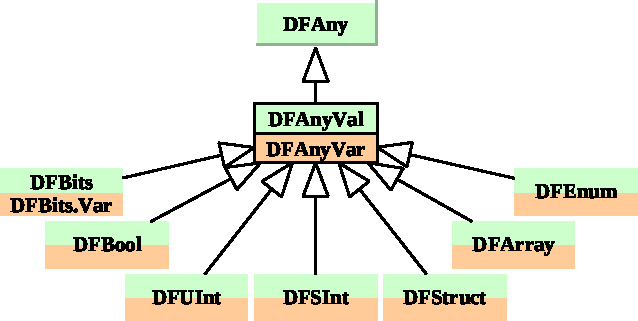
\includegraphics[scale=0.7]{graphics/Inherit.pdf} 
%	\captionof{figure}{DFiant dataflow types: simplified inheritance diagram}
%	\label{fig:Inherit}
%\end{figure}

\subsection{Dataflow Semantics}
DFiant has a dataflow programming model. Data scheduling order, or \textit{token-flow}, is set by the \textit{data dependency}. Essentially, the DFiant semantics schedules all independent dataflow expressions concurrently, while dependent operations are synthesized into a guarded FIFO-styled pipeline. Dataflow branches are implicitly forked and joined. Unused nodes, semantically, always consume tokens, and are discarded during compilation. We observe the DFiant \code{f} implementation as follows:

\begin{enumerate}
  \item All expressions are dataflow variable declarations.
  \item Concurrency is implicit, and \code{f} is coded intuitively, in a sequential manner, since dataflow dependency is oblivious to statement order. 
  \item All scheduling is implicitly guarded by its dependencies. For example, \code{a} is forked into both \code{b} and \code{c} operations, while \code{c} joins branches from \code{a} and \code{b}.
  It is impossible to read an invalid result or an old result (without extending semantics further).
  \item DFiant semantics are intuitive: data is consumed only when it is ready and can be accepted by all receiving nodes, while back-pressure prevents data loss. 
\end{enumerate} 

%The basic DFiant types are DFBits and DFBool
%Each dataflow type points to a static bits vector
%As can be seen from Related Work, HLS "LO TAFAS". Fig. \ref{boxy}
%WE believe one of the primary reasons is that missing features of RTL
%In this section we will cover the RTL features of RTL and how they handled in DFiant's abstractions
%Bring type driven development into hardware design.
%Need inheritance tree.
%Interactions with scala types


\subsection{Bit-Accurate Operations, Type Inference, and Data Structures}
All DFiant's dataflow types are bit-accurate and structurally static, with their bit-width set upon construction (e.g., \code{DFBits[5]} is a 5-bit vector). Operations between dataflow variables produce a bit-accurate result with the proper type inference. For example, an addition between an unsigned 5-bit variable (\code{DFUInt[5]}) and a signed 10-bit variable (\code{DFSInt[10]}) produces an adder that can be implicitly converted to a 10-bit signed variable, if carry is not required, or an 11-bit signed variable by explicitly invoking \code{.wc} from the addition.

DFiant also allows operations between dataflow types and their corresponding Scala numeric types, by treating the Scala numeric types as constants (e.g., addition between \code{DFSInt} and \code{Integer} variables). A constant in the dataflow graph is a node that can produce infinite tokens of the same value.   

\subsection{Mutability}
\label{sec:mutability}
DFiant supports dataflow variables mutability via the \code{:=} operator. Do not confuse with Scala-level mutability which is enabled by using \code{var} instead of \code{val}. Each dataflow class has two variations: an immutable class, which inherits from \code{DFAny\textbf{Val}} and a mutable class, which inherits from \code{DFAny\textbf{Var}} and accepts \code{:=}. The difference between the types enforces an immutable right-hand-side (RHS), where required, and a mutable variable creation. Consider, for instance, the DFiant implementation of \code{g} in Table \ref{tbl:StateExDefImpl}: \code{a} is immutable because it is a RHS addition between the dataflow variable \code{i} and a literal value \code{5}. Contrarily, \code{c} is mutable, since it is a dataflow variable constructor (\code{.init} constructs a new initialized variable, while preserving the mutability trait). 

Fig.~\ref{fig:Inherit} demonstrates a dual class definition for every type  (immutable and mutable). The naming convention helps to reason about the mutability. For example, \code{DFBits} and \code{DFBits.Var} are immutable and mutable classes, respectively. Constructing a new variable via \code{DFBits} (e.g, \code{val a = DFBits[5]}) returns the mutable \code{DFBits.Var[5]}. Usually, we either receive or return an immutable type, hence we do not require annotating a type with its mutable variation. In cases where we want to return a mutable type, we annotate it as an output port (see Section~\ref{sec:io_ports}).

%DFiant's code safety is enforced by maintaining the 'DF-mutability' trait while aliasing (accepting the ':=' operator). This means that an alias of a \textbf{Var}, is still a \textbf{Var}, and can be assigned, while an alias of a \textbf{Val} cannot. This concept is illustrated in ???, and further explained in ???:




\subsection{Bit Aliasing and Casting}
Aliasing in DFiant enables referencing a part of a dataflow variable, by invoking \code{.bits(hiIdx, loIdx)}, which creates a bits vector alias that references the original variable at the given index parameters. Every change of a dataflow variable affects its alias and vice versa (similar to VHDL's signal aliasing). Since this function also casts the variable as \code{DFBits}, this feature is used as a raw-data cast between different dataflow types. Aliasing of an alias is also possible, while maintaining relative bits indexing. Aliasing preserves the mutability trait: an alias of an immutable variable is immutable, while an alias of a mutable variable is mutable. 


Fig.~\ref{fig:Aliasing} demonstrates aliasing code and its effect on the contents of a dataflow variable (\code{bits128}). Each line code does as follows:
\begin{enumerate}
  \item Constructs a new 128-bit vector, \code{bits128}, and clears it.
  \item Creates a new alias, \code{alias64}, which references the most significant 64 bits of \code{bits128}. Since \code{bits128} is a \code{DFBits} variable, there is no need to invoke \code{.bits()}, and we can apply the required indexes directly.
  \item Creates a new alias, \code{alias32}, which references the least significant 32 bits of \code{alias64}, which reference bits 64 to 95 of \code{bits128}.
  \item Constructs a new double precision floating point dataflow variable, \code{dbl}, and initialize its value as \code{1.0} (hexadecimal value of \code{0x3FF00...0}).
  \item Modifies the least significant byte of \code{dbl}.
  \item Sets the most significant bit of \code{bits128}.
  \item Assigns \code{dbl} to the least significant 64 bits of \code{bits128} through casting. All the bits of \code{dbl} are selected because \code{.bits()} is invoked without index parameters.
  \item Modifies a byte of \code{bits128}.
  
\end{enumerate}

\begin{figure}[h]
  \centering
  \begin{minipage}[b][3cm][b]{0.57\linewidth}
    \vfill
    \begin{minted}[xleftmargin=1.5em,linenos,autogobble,tabsize=2,framesep=1pt, frame=single,fontsize=\fontsize{8}{8}\selectfont]{scala}
      val bits128 = DFBits[128] := 0
      val alias64 = bits128(127, 64)
      val alias32 = alias64(31, 0)
      val dbl = DFDouble := 1.0
      dbl.bits(7,0) := 0x28
      bits128(127) := 1
      bits128(63, 0) := dbl.bits()
      alias32(16, 8) := 0x57		    
    \end{minted}
    \vfill
    \subcaption{DFiant code}
  \end{minipage}%
  \hfill
  \begin{minipage}[b][3cm][b]{0.42\linewidth}
    \centering
    \vfill
		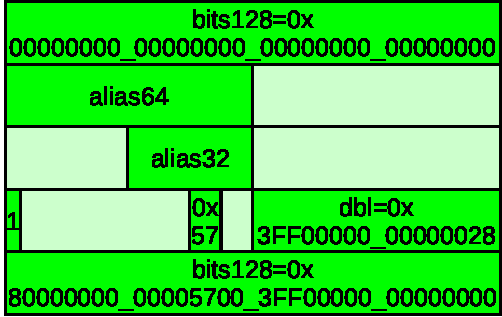
\includegraphics[width=\linewidth]{graphics/Aliasing.pdf} 
    \vfill
    \subcaption{Contents of \code{bits128}}
  \end{minipage}
  \captionof{figure}{Bit aliasing and casting example}
  \label{fig:Aliasing}
\end{figure}


\subsection{Structural Composition and Generation}

DFiant expands traditional structural composition capabilities by utilizing Scala's object oriented features such as inheritance and polymorphism, as well as finite loops and recursive composition. The hierarchical compositions provide the scope and dependencies for the dataflow variables. The hierarchy itself is transparent to the dataflow graph, as if the entire design is flattened, inlined, and unrolled. Therefore, hierarchies in DFiant are synthesizable, highly reusable, and do not affect the design performance (may affect compilation time). Different composition examples are available in Table~\ref{tbl:Box}.

\begin{table*}[t]
  \captionof{table}{DFiant Hierarchy Example: Inheritance, Polymorphism, Recursive Composition, and Inlined View}
  \label{tbl:Box}
  \begin{tabular}{|c|c|c|}
    \hline 
    \textbf{Description} & \textbf{DFiant Code} & \textbf{Functional Drawing} \\ 
    \hline
    \begin{minipage}{0.1\textwidth}
      \footnotesize
      \flushleft
      Abstract base class, \code{Box} (defines only an interface)
    \end{minipage} 
    &
    \begin{minipage}{0.48\textwidth}
      \begin{minted}[autogobble,tabsize=2,framesep=1pt,fontsize=\fontsize{8}{8}\selectfont]{scala}
      type DFB = DFUInt[32] //Type alias, to save code space
      abstract class Box(iT: DFB, iB: DFB) { //T=Top, B=Bottom 
        val oT: DFB
        val oB: DFB
      }
      \end{minted}
    \end{minipage} 
    &  
    \begin{minipage}[c][1.5cm]{0.34\textwidth}
      \centering
      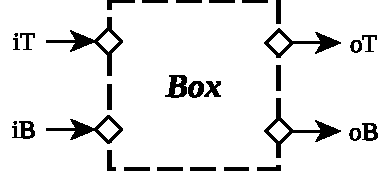
\includegraphics[height=1.3cm]{graphics/Box.pdf}%
    \end{minipage} 
    \\ 
    \hline 
    \begin{minipage}{0.1\textwidth}
      \footnotesize
      \flushleft
      Concrete \code{Box} implementation examples
    \end{minipage} 
    &
    \begin{minipage}{0.48\textwidth}
      \begin{minted}[autogobble,tabsize=2,framesep=1pt,fontsize=\fontsize{8}{8}\selectfont]{scala}
      case class BoxY(iT: DFB, iB: DFB) extends Box(iT, iB) {
        val (oT, oB) = (iT * iT, iT + iB)
      }
      case class BoxE(iT: DFB, iB: DFB) extends Box(iT, iB) {
        val (oT, oB) = (iT + iB, iB)
      }
      \end{minted}
    \end{minipage} 
    &  
    \begin{minipage}[c][1.8cm]{0.34\textwidth}
      \centering
      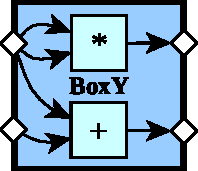
\includegraphics[height=1.3cm]{graphics/BoxY.pdf}%
      \quad\quad\quad
      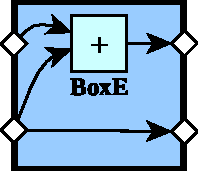
\includegraphics[height=1.3cm]{graphics/BoxE.pdf}%
    \end{minipage} 
    \\ 
    \hline
    \begin{minipage}{0.1\textwidth}
      \footnotesize
      \flushleft
      \code{Box123}, an abstract polymorphic composition of three \code{Box} instances
    \end{minipage} 
    &
    \begin{minipage}{0.48\textwidth}
      \begin{minted}[autogobble,tabsize=2,framesep=1pt,fontsize=\fontsize{8}{8}\selectfont]{scala}
      abstract class Box123(iT: DFB, iB: DFB) extends Box(iT, iB){
        def b1Bld(iT: DFB, iB: DFB) : Box
        def b3Bld(iT: DFB, iB: DFB) : Box
        val b1 = b1Bld(iT,     iB)
        val b2 = BoxE(b1.oB,   b1.oT)
        val b3 = b3Bld(b2.oB,  b2.oT)
        val (oT, oB) = (b3.oT, b3.oB)
      }
      \end{minted}
    \end{minipage} 
    &  
    \begin{minipage}[c][2.3cm]{0.34\textwidth}
      \centering
      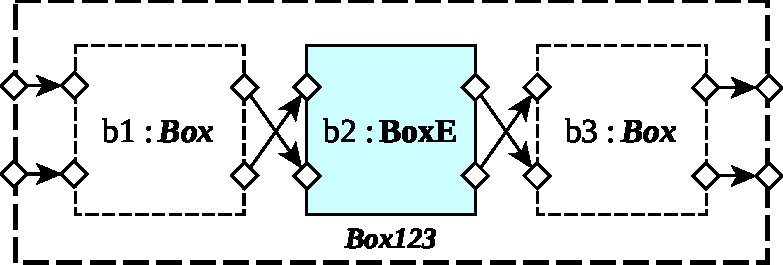
\includegraphics[height=2.1cm]{graphics/Box123.pdf}%
    \end{minipage} 
    \\ 
    \hline
    \begin{minipage}{0.1\textwidth}
      \footnotesize
      \flushleft
      \code{BoxYEE}, a concrete polymorphic composition of three \code{Box} instances \\+\\An inlined view of \code{BoxYEE}
    \end{minipage} 
    &
    \begin{minipage}{0.48\textwidth}
      \begin{minted}[autogobble,tabsize=2,framesep=1pt,fontsize=\fontsize{8}{8}\selectfont]{scala}
      case class BoxYEE(iT: DFB, iB: DFB) extends Box123(iT, iB) {
        def b1Bld(iT: DFB, iB: DFB) = BoxY(iT, iB)
        def b3Bld(iT: DFB, iB: DFB) = BoxE(iT, iB)
      }
      \end{minted}
    \end{minipage} 
    &  
    \begin{minipage}[c][4.6cm]{0.34\textwidth}
      \centering
      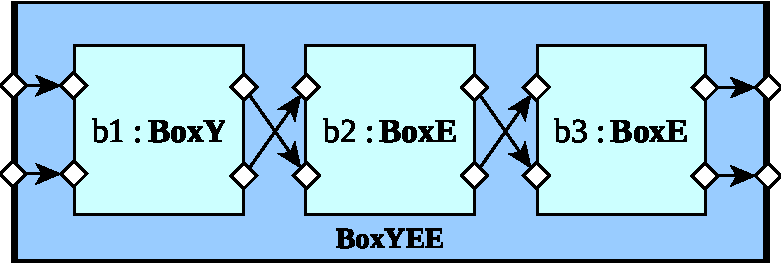
\includegraphics[height=2.1cm]{graphics/BoxYEE.pdf} \\
      \vspace{0.1cm}
      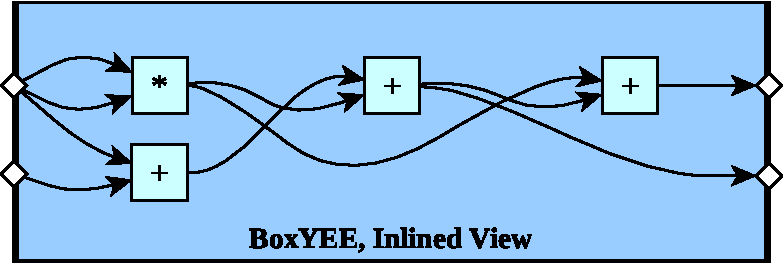
\includegraphics[height=2.1cm]{graphics/BoxYEEInlined.pdf}%
    \end{minipage} 
    \\ 
    \hline
    \begin{minipage}{0.1\textwidth}
      \footnotesize
      \flushleft
      Finite recursive composition example
    \end{minipage} 
    &
    \begin{minipage}{0.48\textwidth}
      \begin{minted}[autogobble,tabsize=2,framesep=1pt,fontsize=\fontsize{8}{8}\selectfont]{scala}
      case class BoxBox(N: Int)(iT: DFB, iB: DFB) 
      extends Box(iT, iB) {
        val b = BoxY(iT, iB)
        val bb : Box = if (N > 0) BoxBox(N - 1)(b.oT, b.oB)
                       else b
        val (oT, oB) = (bb.oT, bb.oB)
      }
      \end{minted}
    \end{minipage} 
    &  
    \begin{minipage}[c][2.3cm]{0.34\textwidth}
      \centering
      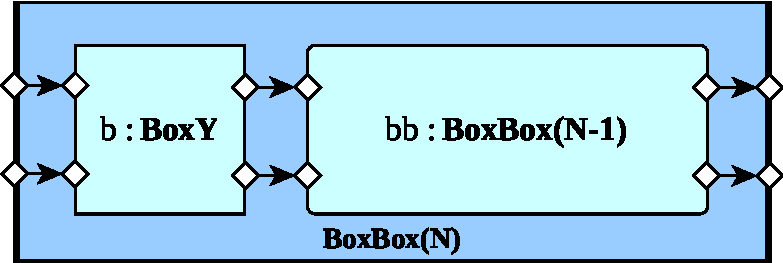
\includegraphics[height=2.1cm]{graphics/BoxBox.pdf}%
    \end{minipage} 
    \\ 
    \hline
  \end{tabular} 
\end{table*}


\subsection{IO Ports}
\label{sec:io_ports}
The class \textit{Box} from Table~\ref{tbl:Box} can also be coded as demonstrated in Fig.~\ref{fig:IOBox}. The annotation \code{DFVar $<>$ Dir} controls \textit{DFVar}'s access by encapsulating the variable with the dataflow port class, \code{DFPort}: an \code{IN} port can only be read (immutable), while an \code{OUT} port can only be modified (unreadable). DFiant has implicit conversions in place that selectively converts between \code{DFPort} and \code{DFAny} instances, without breaking mutability rules and type safety. The port annotations match the capabilities of traditional HDLs, and are noticeably absent from HLS languages such as C++. 


\begin{figure}[h]
  \centering
  \begin{minipage}{0.4\linewidth}
  \begin{minted}[autogobble,tabsize=2,framesep=1pt, frame=single,fontsize=\fontsize{8}{8}\selectfont]{scala}
  abstract class Box() { 
    val iT: DFB <> IN
    val iB: DFB <> IN
    val oT: DFB <> OUT
    val oB: DFB <> OUT
  }
  \end{minted}
  \end{minipage}
  \captionof{figure}{IO port annotation DFiant code example}
  \label{fig:IOBox}
\end{figure}



%+ C has no clear input/output notation. Input array and output array are the same.
%
%+ IDE: Intellisense, error highlighting, code completion, watches, println.
%+ Unified compilation
%+ Complete project build with the IDE. Compile results.
%Yes abstract away pipelining. No to scheduling control.
%
%Features we don't want
%simulations constructs.
%separate constraints file.
%
%VHDL Possible race conditions.
%
%
%+Include a summary table of RTL feature abstraction and how their are defined in DFiant.


  

  \begin{figure}[h]
	\vspace*{-3ex}
	\centering
	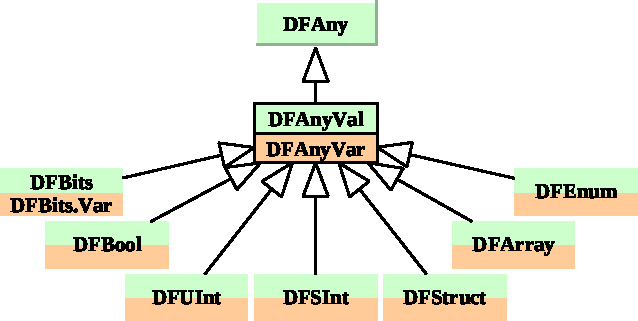
\includegraphics[scale=0.7]{graphics/Inherit.pdf} 
	\captionof{figure}{DFiant dataflow types: simplified inheritance diagram}
	\label{fig:Inherit}
\end{figure}

%\setalgorithmicfont{\small}
\begin{figure*}[h]
  \centering
  \begin{subfigure}[b]{0.5\textwidth}
    \begin{minted}[tabsize=2,gobble=3,frame=single,framesep=2pt, fontsize=\fontsize{7}{8}\selectfont]{Scala}
    class AES_DFKeySchedule(Nk: Int, Nb: Int, Nr : Int) 
      extends AES_DFWords(Nb*(Nr+1)){
      val Rcon = Array[Int](0x00000000, ...)
      def KeyExpansion(key : AES_DFKey): Unit = {
        val temp = AES_DFWord()
      
        for (i <- 0 until Nk)
          this(i) := key(i)
      
      
      
        for (i <- Nk until Nb*(Nr+1)) {
          temp := this(i-1)
          if (i % Nk == 0)
            temp := temp.RotWord().SubWord() ^ Rcon(i / Nk)
          else if ((Nk > 6) && (i % Nk == 4))
            temp := temp.SubWord()
          
          this(i) := this(i-Nk) ^ temp
        
        }
    } }
    \end{minted}
    \caption{DFiant code}
  \end{subfigure}%
%  \hfill
  \begin{subfigure}[b]{0.5\textwidth}
    \begin{minted}[tabsize=2,gobble=3,frame=single,framesep=2pt, fontsize=\fontsize{7}{8}\selectfont]{text}
    //comment line for alignment
    //comment line for alignment
    Rcon = [00000000, ...] 
    KeyExpansion(byte key[4*Nk], word w[Nb*(Nr+1)], Nk) begin
      word temp
      i = 0
      while (i < Nk)
        w[i] = word(key[4*i],key[4*i+1],key[4*i+2],key[4*i+3])
        i = i+1
      end while
      i = Nk
      while (i < Nb * (Nr+1)]
        temp = w[i-1]
        if (i mod Nk = 0)
          temp = SubWord(RotWord(temp)) xor Rcon[i/Nk]
        else if (Nk > 6 and i mod Nk = 4)
          temp = SubWord(temp)
        end if
        w[i] = w[i-Nk] xor temp
        i = i + 1
      end while
    end
    \end{minted}
    \caption{AES spec. pseudo code reference}
  \end{subfigure}
	\vspace*{-4ex}
  \caption{AES KeyExpansion code example}\label{fig:AES}
\end{figure*}

\section{The DFiant Type System}
\label{sec:type_system}
DFiant is a Scala library, hence it inherently supports type safe and rich language constructs. DFiant brings type driven development concepts to hardware design, by creating an extensible dataflow class hierarchy, with the trait \code{DFAny} at its head. 
%(similar concept to Scala's Unified Types hierarchy)
\code{DFAny} contains all properties that are common to every dataflow variable. 
%(e.g., \code{.width} represents the number of bits contained by the variable)
Fig.~\ref{fig:Inherit} illustrates a simplified inheritance diagram of DFiant's dataflow types. 

Fig.~\ref{fig:AES} depicts part of our DFiant Advanced Encryption Standard~\cite{pub2001197} (AES) cipher implementation alongside its specification pseudo code reference. The DFiant code is similar or even simpler in comparison and does not employ global functions. We compared the complete DFiant AES code to three RTL designs~\cite{das2010fully}\cite{hsing2013aes}\cite{salah2013aespipe}. DFiant provides the same functionality with 33-50\% lines of code.
Furthermore, the DFiant code is timing-agnostic and device-agnostic, thus tasking the compiler to construct the hardware fitting the target device and non-functional requirements (e.g., throughput, latency). When constrained by the appropriate target throughput, the DFiant compiler generated an RTL design that acheived better performance than the cited RTL designs.

%Since DFiant is Scala-based, the Scala IDE was utlized for debugging. It was also extremely easy to debug the code step-by-step using
%watches and console printouts. This would have been impossible to do in native HDL
%languages like VHDL and Verilog. After we fixed everything to work in software debugging backend, we have compiled the design to verilog using the hardware construction
%backend, and everything worked in RTL simulation as well.


%The DFiant type system provides the following features:
%\paragraph*{\bf \em Bit-Accurate Operations and Data Structures} 
%All DFiant's dataflow types are bit-accurate and structurally static, with their bit-width set upon construction (e.g., \code{DFBits[5]} is a 5-bit vector). Operations between dataflow variables produce a bit-accurate result with the proper type inference. For example, an addition between an unsigned 5-bit variable (\code{DFUInt[5]}) and a signed 10-bit variable (\code{DFSInt[10]}) produces an adder that can be implicitly converted to a 10-bit signed variable, if carry is not required, or an 11-bit signed variable by explicitly invoking \code{.wc} from the addition.
%
%DFiant also allows operations between dataflow types and their corresponding Scala numeric types, by treating the Scala numeric types as constants (e.g., addition between \code{DFSInt} and \code{Integer} variables). A constant in the dataflow graph is a node that can produce infinite tokens of the same value.   
%
%\paragraph*{\bf \em Mutability} 
%\label{sec:mutability}
%DFiant supports dataflow variables mutability via the \code{:=} operator. Do not confuse with Scala-level mutability which is enabled by using \code{var} instead of \code{val}. Each dataflow class has two variations: an immutable class, which inherits from \code{DFAny\textbf{Val}} and a mutable class, which inherits from \code{DFAny\textbf{Var}} and accepts \code{:=}. The difference between the types enforces an immutable right-hand-side (RHS), where required, and a mutable variable creation. Consider, for instance, the DFiant implementation of \code{g} in Table \ref{tbl:StateExDefImpl}: \code{a} is immutable because it is a RHS addition between the dataflow variable \code{i} and a literal value \code{5}. Contrarily, \code{c} is mutable, since it is a dataflow variable constructor (\code{.init} constructs a new initialized variable, while preserving the mutability trait). 
%
%Fig.~\ref{fig:Inherit} demonstrates a dual class definition for every type  (immutable and mutable). The naming convention helps to reason about the mutability. For example, \code{DFBits} and \code{DFBits.Var} are immutable and mutable classes, respectively. Constructing a new variable via \code{DFBits} (e.g, \code{val a = DFBits[5]}) returns the mutable \code{DFBits.Var[5]}. Usually, we either receive or return an immutable type, hence we do not require annotating a type with its mutable variation. In cases where we want to return a mutable type, we annotate it as an output port (see Section~\ref{sec:io_ports}).
%
%\paragraph*{\bf \em Bit Aliasing and Casting} 
%Aliasing in DFiant enables referencing a part of a dataflow variable, by invoking \code{.bits(hiIdx, loIdx)}, which creates a bits vector alias that references the original variable at the given index parameters. Every change of a dataflow variable affects its alias and vice versa (similar to VHDL's signal aliasing). Since this function also casts the variable as \code{DFBits}, this feature is used as a raw-data cast between different dataflow types. Aliasing of an alias is also possible, while maintaining relative bits indexing. Aliasing preserves the mutability trait: an alias of an immutable variable is immutable, while an alias of a mutable variable is mutable. 
%
%\paragraph*{\bf \em Structural Composition and Generation} 
%
%\begin{figure}[h]
%  \centering
%  \begin{minipage}[b][3cm][b]{0.57\linewidth}
%    \vfill
%    \begin{minted}[xleftmargin=1.5em,linenos,autogobble,tabsize=2,framesep=1pt, frame=single,fontsize=\fontsize{7}{8}\selectfont]{scala}
%      val bits128 = DFBits[128] := 0
%      val alias64 = bits128(127, 64)
%      val alias32 = alias64(31, 0)
%      val dbl = DFDouble := 1.0
%      dbl.bits(7,0) := 0x28
%      bits128(127) := 1
%      bits128(63, 0) := dbl.bits()
%      alias32(16, 8) := 0x57		    
%    \end{minted}
%    \vfill
%    \subcaption{DFiant code}
%  \end{minipage}%
%  \hfill
%  \begin{minipage}[b][3cm][b]{0.40\linewidth}
%    \centering
%    \vfill
%		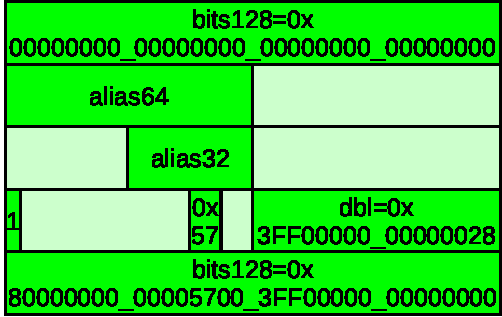
\includegraphics[width=\linewidth]{graphics/Aliasing.pdf} 
%    \vfill
%    \subcaption{Contents of \code{bits128}}
%  \end{minipage}
%  \captionof{figure}{Bit aliasing and casting example}
%  \label{fig:Aliasing}
%\end{figure}
%
%Fig.~\ref{fig:Aliasing} demonstrates aliasing code and its effect on the contents of a dataflow variable (\code{bits128}). Each line code does as follows:
%\begin{enumerate}
%  \item Constructs a new 128-bit vector, \code{bits128}, and clears all its bits.
%  \item Creates a new alias, \code{alias64}, which references the most significant 64 bits of \code{bits128}. Since \code{bits128} is a \code{DFBits} variable, there is no need to invoke \code{.bits()}, and we can apply the required indexes directly.
%  \item Creates a new alias, \code{alias32}, which references the least significant 32 bits of \code{alias64}, which reference bits 64 to 95 of \code{bits128}.
%  \item Constructs a new double precision floating point dataflow variable, \code{dbl}, and initialize its value as \code{1.0} (hexadecimal value of \code{0x3FF00...0}).
%  \item Modifies the least significant byte of \code{dbl}.
%  \item Sets the most significant bit of \code{bits128}.
%  \item Assigns \code{dbl} to the least significant 64 bits of \code{bits128} through casting. All the bits of \code{dbl} are selected because \code{.bits()} is invoked without index parameters.
%  \item Modifies a byte of \code{bits128}.
%  
%\end{enumerate}
%
%
%DFiant expands traditional structural composition capabilities by utilizing Scala's object oriented features such as inheritance and polymorphism, as well as finite loops and recursive composition. The hierarchical compositions provide the scope and dependencies for the dataflow variables. The hierarchy itself is transparent to the dataflow graph, as if the entire design is flattened, inlined, and unrolled. Therefore, hierarchies in DFiant are synthesizable, highly reusable, and do not affect the design performance (may affect compilation time). Different composition examples are available in Table~\ref{tbl:Box}.
%
%\paragraph*{\bf \em IO Ports} 
%\label{sec:io_ports}
%The class \textit{Box} from Table~\ref{tbl:Box} can also be coded as demonstrated in Fig.~\ref{fig:IOBox}. The annotation \code{DFVar $<>$ Dir} controls \textit{DFVar}'s access by encapsulating the variable with the dataflow port class, \code{DFPort}: an \code{IN} port can only be read (immutable), while an \code{OUT} port can only be modified (unreadable). DFiant has implicit conversions in place that selectively converts between \code{DFPort} and \code{DFAny} instances, without breaking mutability rules and type safety. The port annotations match the capabilities of traditional HDLs, and are noticeably absent from HLS languages such as C++. 



  
  
%  \section{Proof of Concept}
\label{sec:evaluation}
In this section we demonstrate DFiant frontend and backend compilers as a proof of concept the preliminary semantics of DFiant by implementing two case studies: an AES cypher, and a double precision FPMul. We compare both test cases against traditional designs, and demonstrate competing performance while simplifying code verbosity significantly. 

\subsection{Methodology}
We implemented both test cases in DFiant, constrained them by a variance of minimum frequency requirements, and compiled them to RTL. The DFiant compiler automatically pipelined the design to achieve the required minimum frequency, and generated an RTL verilog file and a TCL constraints file. For a baseline we obtained equivalent open-source RTL cores and Vivado HLS implementations, where possible. We disabled the DFiant backend support for pipelined valid/ready signaling and a blocking back-pressure, since the RTL cores did not support this capability.

We chose the following comparison metrics: the maximum clock frequency, clock cycle latency, utilizations of both look-up tables (LUTs) and flip-flop registers (FFs), and lines of code (LoC). Digital signal processing (DSP) block utilization was zero for AES and equivalent for FPMul across all designs, thus neglected from the table. a We used Xilinx Vivado to synthesize and implement the RTL design for a Virtex-7 FPGA, part number: xc7vx485tffg1761-2. The tool was configured to use default strategy for both synthesis and implementation processes. For each design, we recorded the maximum clock frequency, LUTs, and FFs. We recorded the design latency as reported by the DFiant and Vivado HLS compilers, and the RTL cores documentation. Finally, we automatically counted the LoC \cite{danial2009cloc}, applied standard score normalization (0-100) to all metrics, and assured higher values indicate better score for all metrics. Mean score of all metrics is presented as well.

\subsection{Case Study: AES Cypher}
For baseline comparison we used three AES cypher RTL designs from opencores.org: Das core \cite{das2010fully}, Hsing core \cite{hsing2013aes} and Salah core \cite{salah2013aespipe}. Additionally, we obtained a Vivado C++ HLS design~\cite{oflynn2014rapid}. All these designs are fully pipelined, meaning that in every cycle the design accepts new key and data inputs, and emits an encrypted data output, delayed by a fixed design latency.

We compiled the DFiant and Vivado HLS designs with three target clock frequencies: 200 MHz, 300 MHz, and 450 MHz. We named the designs accordingly (e.g., DFiant\_200 is the 200MHz target design). We collected the results in Table~\ref{tbl:AES_Compare_Table}, and displayed their normalized standard score in Fig.~\ref{fig:AES_Compare_Graph}. We added the supported key types quantity as a metric, since some designs support 128bit keys and do not include 192bit and 256bit keys as well. The table also includes an 'SBox BRAM Use' column, since some designs do not use memory to implement the AES SBox function.

\begin{table*}[t!]
  \centering
  \begin{minipage}[t][5cm][t]{0.62\linewidth}
    \centering
    \captionof{table}{AES Cypher RTL Designs Comparison\\(the numbering on the left associates configurations with \fig{fig:AES_Compare_Graph})}
    \label{tbl:AES_Compare_Table}
    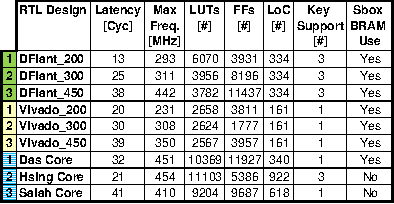
\includegraphics[scale=1]{graphics/AES_Compare_Table.pdf} 
  \end{minipage}
  \hfill
  \begin{minipage}[t][5cm][t]{0.37\linewidth}
    \centering
    \captionof{table}{FP Mult. RTL Designs Comparison\\(the numbering on the left associates configurations with \fig{fig:FP_Compare_Graph})}
    \label{tbl:FP_Compare_Table}
    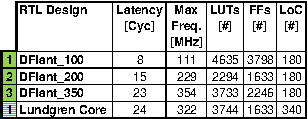
\includegraphics[scale=1]{graphics/FP_Compare_Table.pdf} 
  \end{minipage}
  \begin{minipage}[b][3.8cm][b]{0.62\linewidth}
  	\centering
    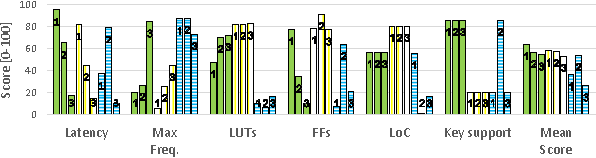
\includegraphics[height=3cm]{graphics/AES_Compare.pdf} 
    \captionof{figure}{AES cypher RTL designs score comparison (higher = better)\\ \quad}
    \label{fig:AES_Compare_Graph}
  \end{minipage}
  \hfill
  \begin{minipage}[b][3.8cm][b]{0.37\linewidth}
    \centering
    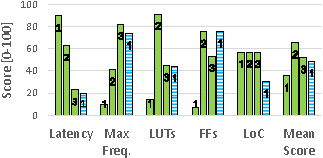
\includegraphics[height=3cm]{graphics/FP_Compare.pdf} 
    \captionof{figure}{FP multiplication RTL designs score comparison (higher = better)}
    \label{fig:FP_Compare_Graph}
  \end{minipage}
\end{table*}

The Hsing core clearly has the best performance among the different designs (but the lowest score on LUTs utilization). The primary reason it achieved this is because it uses LUTs instead of BRAMs. This enables the synthesizer to optimize the AES SBox function, and even pipeline it. DFiant uses its \code{lookupTable} library function to implement SBox, and we have yet to enable such an option for DFiant. 

Although the DFiant-generated RTL performance is not optimal, it can still  be improved without modifying the DFiant AES code, if the DFiant compiler is optimized. Moreover, this code has an adaptive pipeline, while the RTL cores pipelines are fixed. The Vivado implementation enjoys the same advantages as DFiant, and has even less LoC. However, the Vivado code does not support all possible keys and its maximum performance is far from optimum (we did not attempt to improve the HLS pragma directives).

If we assume all metrics have the same weight, the mean score places the DFiant solutions at the top. It is difficult to determine what is truly the best solution, but DFiant clearly has the best potential for further improvement without any modification to the application code.

           
\subsection{Case Study: Double Precision FPMul}

We compared our FPMul with the open IEEE-754 compatible Lundgren core \cite{lundgren2014open} (the only IEEE-754 fully compatible FPMul RTL design we had access to). Since the core is a complete floating point unit, we disabled the unnecessary parts, reducing it to only an FPMul, for a fair comparison with DFiant's code. The DFiant code was written by using the Lundgren VHDL code as a reference design. The designs are very similar in their structure, except that DFiant is considerably less verbose, and has no explicit pipeline.

We had no access to an open Vivado HLS FPMul for comparison. We could have directly invoked a \textit{double} multiplication, but an inspection of the generated RTL revealed that Vivado HLS just instantiates an RTL floating point blackbox core. DFiant can choose to use this core as well, and achieve identical performance to Vivado HLS. Furthermore, the Vivado HLS floating point implementation is not fully compatible with IEEE-754 (e.g, does not support denormalized numbers).

Similarly to the AES case study, we collected the results in Table~\ref{tbl:FP_Compare_Table}, and displayed their normalized standard score in Fig.~\ref{fig:FP_Compare_Graph}. In comparison with the Lundgren core, DFiant\_350 is better in every criteria, aside from FFs utilization. Ultimately, DFiant out-performs its reference design of FPMul, and demonstrates its ability to provide different RTL designs for design space exploration.


  
  
  \section{Conclusion}
\label{sec:conclusion}
In this paper we presented our extension of DFiant, a dataflow HDL, and exposed its advantageous semantics, when compared to modern RTLs and C++-based HLS tools, such as VHDL and Vivado HLS, respectively. DFiant provides a seamless concurrent programming approach, and yet it still facilitates a versatile compositional and hierarchical expressiveness. We evaluated DFiant in two computational-heavy case studies, and demonstrated its competing performance alongside its code simplification. 

%Although we established its many benefits, DFiant is still missing a few milestones before it becomes a worthy replacement for the traditional HDLs. 
So far,  we demonstrated how DFiant covers static one-to-one token transfer functions. Notwithstanding, functionality may require upsampling (e.g., duplicate each token), downsampling (e.g., drop every third token), token arrival time dependency (e.g., priority round-robin arbiter), or token value dependency (e.g., filter out odd-valued tokens). Future work may explore expanding control over token generation and consumption.


%We continued the work of Port & Etsion
%New approach by Port and Etsion \cite{port2015} %Our previous work%
%suggests. 


	
	% An example of a floating figure using the graphicx package.
	% Note that \label must occur AFTER (or within) \caption.
	% For figures, \caption should occur after the \includegraphics.
	% Note that IEEEtran v1.7 and later has special internal code that
	% is designed to preserve the operation of \label within \caption
	% even when the captionsoff option is in effect. However, because
	% of issues like this, it may be the safest practice to put all your
	% \label just after \caption rather than within \caption{}.
	%
	% Reminder: the "draftcls" or "draftclsnofoot", not "draft", class
	% option should be used if it is desired that the figures are to be
	% displayed while in draft mode.
	%
%	\begin{figure}[!t]
%	\centering
%%			\inputminted{Scala}{graphics/BoxyCode.scala}
%%	\includegraphics[width=2.5in]{graphics/Boxy.pdf}
%	\caption{Simulation results for the network.}
%	\label{fig_sim}
%	\end{figure}
	
	% Note that the IEEE typically puts floats only at the top, even when this
	% results in a large percentage of a column being occupied by floats.
	
	
	% An example of a double column floating figure using two subfigures.
	% (The subfig.sty package must be loaded for this to work.)
	% The subfigure \label commands are set within each subfloat command,
	% and the \label for the overall figure must come after \caption.
	% \hfil is used as a separator to get equal spacing.
	% Watch out that the combined width of all the subfigures on a 
	% line do not exceed the text width or a line break will occur.
	%
%	\begin{figure*}[!t]
%	\centering
%	\subfloat[Case I]{\includegraphics[width=2.5in]{graphics/Boxy.pdf}%
%	\label{fig_first_case}}
%	\hfil
%	\subfloat[Case II]{\includegraphics[width=2.5in]{graphics/Boxy.pdf}%
%	\label{fig_second_case}}
%	\caption{Simulation results for the network.}
%	\label{fig_sim}
%	\end{figure*}
	%
	% Note that often IEEE papers with subfigures do not employ subfigure
	% captions (using the optional argument to \subfloat[]), but instead will
	% reference/describe all of them (a), (b), etc., within the main caption.
	% Be aware that for subfig.sty to generate the (a), (b), etc., subfigure
	% labels, the optional argument to \subfloat must be present. If a
	% subcaption is not desired, just leave its contents blank,
	% e.g., \subfloat[].
	
	
	% An example of a floating table. Note that, for IEEE style tables, the
	% \caption command should come BEFORE the table and, given that table
	% captions serve much like titles, are usually capitalized except for words
	% such as a, an, and, as, at, but, by, for, in, nor, of, on, or, the, to
	% and up, which are usually not capitalized unless they are the first or
	% last word of the caption. Table text will default to \footnotesize as
	% the IEEE normally uses this smaller font for tables.
	% The \label must come after \caption as always.
	%
	%\begin{table}[!t]
	%% increase table row spacing, adjust to taste
	%\renewcommand{\arraystretch}{1.3}
	% if using array.sty, it might be a good idea to tweak the value of
	% \extrarowheight as needed to properly center the text within the cells
	%\caption{An Example of a Table}
	%\label{table_example}
	%\centering
	%% Some packages, such as MDW tools, offer better commands for making tables
	%% than the plain LaTeX2e tabular which is used here.
	%\begin{tabular}{|c||c|}
	%\hline
	%One & Two\\
	%\hline
	%Three & Four\\
	%\hline
	%\end{tabular}
	%\end{table}
	
	
	% Note that the IEEE does not put floats in the very first column
	% - or typically anywhere on the first page for that matter. Also,
	% in-text middle ("here") positioning is typically not used, but it
	% is allowed and encouraged for Computer Society conferences (but
	% not Computer Society journals). Most IEEE journals/conferences use
	% top floats exclusively. 
	% Note that, LaTeX2e, unlike IEEE journals/conferences, places
	% footnotes above bottom floats. This can be corrected via the
	% \fnbelowfloat command of the stfloats package.
	
	

	
	
	% conference papers do not normally have an appendix
	
	
	% use section* for acknowledgment
%	\section*{Acknowledgment}
%	
%	
%	The authors would like to thank the Scala community; a great compiler with great libraries made by great people.
	
	
	
	
	
	% trigger a \newpage just before the given reference
	% number - used to balance the columns on the last page
	% adjust value as needed - may need to be readjusted if
	% the document is modified later
	%\IEEEtriggeratref{8}
	% The "triggered" command can be changed if desired:
	%\IEEEtriggercmd{\enlargethispage{-5in}}
	
	% references section
	
	% can use a bibliography generated by BibTeX as a .bbl file
	% BibTeX documentation can be easily obtained at:
	% http://mirror.ctan.org/biblio/bibtex/contrib/doc/
	% The IEEEtran BibTeX style support page is at:
	% http://www.michaelshell.org/tex/ieeetran/bibtex/
	\bibliographystyle{IEEEtran}
	% argument is your BibTeX string definitions and bibliography database(s)
	\bibliography{bib/macros,bib/references}
	%
	% <OR> manually copy in the resultant .bbl file
	% set second argument of \begin to the number of references
	% (used to reserve space for the reference number labels box)
%	\begin{thebibliography}{1}
%		
%		\bibitem{IEEEhowto:kopka}
%		H.~Kopka and P.~W. Daly, \emph{A Guide to \LaTeX}, 3rd~ed.\hskip 1em plus
%		0.5em minus 0.4em\relax Harlow, England: Addison-Wesley, 1999.
%		
%	\end{thebibliography}
	
	
	
	
	% that's all folks
\end{document}


\grid
